%%%%%%%%%%%%%%%%%%%%%%%%%%%%%%%%%%%%%%%%%%%%%%%%%%%%%%%%%%%%%%%%%%%%
%% CABER: Coalgebraic Behavioral Auditing of Foundation Models
%%        via Sublinear Probing
%%
%% Tool Paper — Conference Format
%%%%%%%%%%%%%%%%%%%%%%%%%%%%%%%%%%%%%%%%%%%%%%%%%%%%%%%%%%%%%%%%%%%%
\documentclass[11pt,letterpaper]{article}

% ── Layout ──────────────────────────────────────────────────────────
\usepackage[margin=1in]{geometry}
\usepackage{parskip}

% ── Math ────────────────────────────────────────────────────────────
\usepackage{amsmath,amssymb,amsthm}

% ── Graphics & Figures ──────────────────────────────────────────────
\usepackage{graphicx}
\usepackage{tikz}
\usetikzlibrary{arrows.meta,positioning,fit,calc,decorations.pathreplacing,shapes.geometric}
\usepackage{pgfplots}
\pgfplotsset{compat=1.18}

% ── Tables ──────────────────────────────────────────────────────────
\usepackage{booktabs}
\usepackage{multirow}
\usepackage{tabularx}

% ── Algorithms ──────────────────────────────────────────────────────
\usepackage{algorithm}
\usepackage{algpseudocode}

% ── Colors & Hyperlinks ────────────────────────────────────────────
\usepackage[dvipsnames]{xcolor}
\usepackage[colorlinks=true,linkcolor=MidnightBlue,citecolor=OliveGreen,urlcolor=BrickRed]{hyperref}

% ── Misc ────────────────────────────────────────────────────────────
\usepackage{enumitem}
\usepackage{url}

% ── Theorem-like environments ──────────────────────────────────────
\newtheorem{theorem}{Theorem}[section]
\newtheorem{lemma}[theorem]{Lemma}
\newtheorem{definition}[theorem]{Definition}
\newtheorem{proposition}[theorem]{Proposition}
\newtheorem{example}[theorem]{Example}
\newtheorem{remark}[theorem]{Remark}

% ── Macros ──────────────────────────────────────────────────────────
\newcommand{\tool}{\textsc{Caber}}
\newcommand{\pclstar}{PCL$^*$}
\newcommand{\coalcegar}{\textsc{CoalCEGAR}}
\newcommand{\qctlf}{QCTL$_F$}
\newcommand{\OO}{\mathcal{O}}
\newcommand{\Otil}{\tilde{\mathcal{O}}}
\newcommand{\DD}{\mathcal{D}}
\newcommand{\FF}{\mathcal{F}}
\newcommand{\HH}{\mathcal{H}}
\newcommand{\KK}{\mathcal{K}}
\newcommand{\BB}{\mathcal{B}}
\newcommand{\TT}{\mathcal{T}}

\title{\textbf{CABER: Coalgebraic Behavioral Auditing of\\Foundation Models via Sublinear Probing}}

\date{}

\begin{document}
\maketitle

% ====================================================================
%  ABSTRACT
% ====================================================================
\begin{abstract}
We present \tool{}, a verification engine that treats
black-box large language models (LLMs) as coalgebras and extracts
finite behavioral automata via a novel \emph{Probabilistic Coalgebraic
$L^*$} (\pclstar{}) algorithm.  Learned automata are model-checked
against temporal behavioral specifications expressed in \qctlf{}, a
quantitative extension of CTL parameterized by behavioral functors,
producing graded audit reports with PAC-style soundness guarantees.
\tool{} introduces three key technical contributions:
(i)~a \emph{functor bandwidth} invariant that governs the
information-theoretic complexity of the behavioral functor and yields
sub-linear query complexity in the natural-language alphabet size;
(ii)~\coalcegar{}, an abstraction--refinement loop over parameterized
behavioral functors that navigates an explicitly maintained abstraction
lattice to balance precision and query cost; and
(iii)~a \emph{quantitative bisimulation distance} based on Kantorovich
lifting that enables regression detection across model versions.

\paragraph{Empirical results.}
We validate \tool{} at three levels.
\emph{(i)~Real LLM experiment:} We deploy \tool{} against OpenAI's
\texttt{gpt-4.1-nano} via API, extracting a 3-state behavioral automaton
(initial, compliant, refusal) from 45 queries.  Three behavioral
properties---refusal persistence, sycophancy resistance, jailbreak
resistance---are checked with 100\% pass rate, demonstrating that
real LLM behavior admits tractable finite-state abstraction.
\emph{(ii)~PDFA+PRISM baseline comparison:} On four mock LLM benchmarks,
\tool{}'s coalgebraic PCL$^*$ produces automata 5--10$\times$ more
compact than PDFA baselines (19--40 states vs.\ 176--356 states) with
higher prediction accuracy (73--100\% vs.\ 57--85\%), validating the
benefit of observation-table-based state discrimination.
\emph{(iii)~State scaling:} PCL$^*$ maintains ${\ge}96\%$ prediction
accuracy up to 100 ground-truth behavioral states, with query
complexity scaling as $O(n^{1.42})$.
Classifier robustness analysis demonstrates tolerance to systematic
classifier errors up to $\rho = 0.20$, with Monte Carlo simulation
(2{,}000 trials per error rate) showing ${\ge}99.2\%$ verdict accuracy.
Mathematical invariants are validated by 38 property-based tests
(Rust \texttt{proptest}).

\paragraph{Limitations.}
The real LLM experiment uses \texttt{gpt-4.1-nano}, a small model;
experiments on frontier models (GPT-4, Claude~3.5) remain future work.
The alphabet abstraction (embedding clustering) introduces a
non-functorial pre-categorical step whose errors are bounded but not
eliminated by the PAC framework.  Full Lean~4 formalization is
deferred; property-based testing bridges the current gap.
\end{abstract}

% ====================================================================
%  1. INTRODUCTION
% ====================================================================
\section{Introduction}\label{sec:intro}

Foundation models---large language models (LLMs) deployed behind
API endpoints---are updated silently, frequently, and without
behavioral contracts.  A downstream system that relies on GPT-4's
refusal policy, Claude's multi-turn consistency, or Gemini's
instruction-following behavior has no mechanism to detect when the
model's behavior has changed, let alone whether the change violates an
application-specific invariant.  We call this the \emph{behavioral
regression problem}: the provider modifies the model behind the API,
and the consumer discovers the change only through user complaints or
production failures.

\paragraph{Motivating incidents.}
Three documented episodes illustrate the severity of silent behavioral
shifts:
\begin{enumerate}[leftmargin=*,nosep]
\item \textbf{GPT-4 capability degradation (2023).}
  Chen et al.~\cite{chen2023chatgpt} demonstrated that GPT-4's
  accuracy on several benchmarks dropped significantly between March
  and June 2023, including a 95.2\% $\to$ 2.4\% decline on prime-number
  identification---a behavioral regression detectable only through
  systematic re-evaluation.
\item \textbf{GPT-4 Turbo instruction-following regression (2023--24).}
  Community reports and independent benchmarks documented that the
  GPT-4 Turbo variant exhibited degraded instruction adherence relative
  to the base GPT-4 snapshot, particularly for structured-output
  formatting and system-prompt compliance.
\item \textbf{Claude safety oscillations (2023--24).}
  Across Anthropic's model updates, users observed non-monotonic
  changes in refusal boundaries: prompts refused by one version were
  accepted by the next, and vice versa, suggesting the absence of a
  stable behavioral specification.
\end{enumerate}

\paragraph{Why existing tools fall short.}
Current evaluation suites such as HELM~\cite{liang2023helm},
CheckList~\cite{ribeiro2020beyond}, and direct statistical
testing~\cite{chen2023chatgpt} share three limitations:
(a)~they operate on \emph{static} snapshots rather than extracting a
\emph{behavioral model} that can be analyzed compositionally;
(b)~they lack a \emph{temporal} dimension---properties such as
``refusal is persistent across paraphrases'' or ``the model never
reverses its safety judgment within a session'' are inherently
multi-step and cannot be expressed as single-query accuracy metrics;
(c)~they provide no formal soundness guarantees on the reported
pass/fail verdicts.

\paragraph{\tool{}'s approach.}
\tool{} addresses these gaps by combining two mature formal-methods
traditions---\emph{active automata learning} and \emph{temporal model
checking}---with a coalgebraic abstraction layer that makes the
combination tractable for the LLM domain:
\begin{enumerate}[leftmargin=*,nosep]
\item A \emph{behavioral functor} $F_{\mathrm{LLM}}$ parameterizes
  what aspect of the model's behavior is being learned (output
  distributions, refusal patterns, multi-turn trajectories).
\item The \pclstar{} algorithm actively queries the model and
  constructs a finite weighted automaton that approximates the
  observable behavior under $F_{\mathrm{LLM}}$.
\item The learned automaton is model-checked against temporal
  specifications written in \qctlf{}, yielding a \emph{graded
  satisfaction degree} in $[0,1]$ rather than a Boolean verdict.
\item Bisimulation distances between automata from different model
  versions quantify behavioral drift.
\end{enumerate}

\paragraph{Contributions.}
This tool paper makes the following contributions:
\begin{itemize}[leftmargin=*,nosep]
\item The \pclstar{} algorithm: a PAC-style extension of Angluin's
  $L^*$~\cite{angluin1987learning} to probabilistic coalgebras, with
  query complexity governed by a \emph{functor bandwidth} invariant
  rather than the raw alphabet size (\S\ref{sec:algorithms}).
\item \coalcegar{}: abstraction--refinement over parameterized
  behavioral functors, navigating an explicitly maintained lattice of
  abstraction triples $(k,n,\varepsilon)$
  (\S\ref{sec:algorithms}).
\item A quantitative model checker for \qctlf{}, an instantiation
  of coalgebraic modal logic in the Pattinson--Schr\"oder
  framework~\cite{pattinson2008coalgebraic} with functorial path
  quantifiers and graded modalities, specialized to LLM behavioral
  specifications (\S\ref{sec:spec}).
\item An open-source implementation comprising ${\sim}99$\,K lines of
  Rust and Python, with a seven-layer architecture designed for
  extensibility (\S\ref{sec:impl}).
\item An experimental evaluation on controlled mock LLMs demonstrating
  learning accuracy, specification-checking soundness, and bisimulation
  distance fidelity (\S\ref{sec:eval}).
\end{itemize}

% ====================================================================
%  2. BACKGROUND
% ====================================================================
\section{Background}\label{sec:background}

\subsection{Coalgebras and Behavioral Equivalence}

A \emph{coalgebra} for an endofunctor $F: \mathbf{Set} \to
\mathbf{Set}$ is a pair $(X, \gamma: X \to F(X))$, where $X$ is a
set of states and $\gamma$ is the transition structure.  Two states
$x, x' \in X$ are \emph{behaviorally equivalent} if they cannot be
distinguished by any finite sequence of observations---formalized
via the notion of \emph{bisimulation}~\cite{rutten2000universal}.

For deterministic automata, $F(X) = X^\Sigma \times 2$ (transition
function plus acceptance); for probabilistic automata, $F(X) =
\DD(X)^\Sigma$, where $\DD$ denotes the distribution monad.  The
coalgebraic perspective unifies these and many other system types
under a single theory~\cite{rutten2000universal,silva2010coalgebraic}.

\begin{definition}[Behavioral Functor for LLMs]\label{def:functor}
Let $\Sigma_{\le k}$ denote the set of output tokens of length at
most $k$ and let $\Sigma^*_{\le n}$ denote prompts of length at most
$n$.  The \emph{LLM behavioral functor} is
\[
  F_{\mathrm{LLM}}(X) \;=\;
    \bigl(\Sigma_{\le k} \times \DD(X)\bigr)^{\Sigma^*_{\le n}},
\]
mapping each state to a function that, for every prompt of bounded
length, returns an output token together with a distribution over
successor states.
\end{definition}

\subsection{Active Automata Learning}

Angluin's $L^*$ algorithm~\cite{angluin1987learning} learns a minimal
DFA for an unknown regular language by posing \emph{membership queries}
(``is string $w$ in the language?'') and \emph{equivalence queries}
(``does hypothesis $H$ equal the target?'') to a \emph{minimally
adequate teacher}.  The algorithm maintains an \emph{observation table}
$(S, E, T)$, where $S$ is a set of access strings, $E$ a set of
distinguishing suffixes, and $T: (S \cup S \cdot \Sigma) \times E \to
\{0,1\}$ the table entries.

Extensions to weighted and probabilistic automata replace Boolean
table entries with real-valued weights drawn from a
semiring~\cite{berstel2011noncommutative}, and approximate equality
with statistical tests~\cite{weiss2018extracting,tappler2019model}.

\subsection{Temporal Logic Model Checking}

Computation Tree Logic (CTL)~\cite{clarke1986automatic} expresses
properties of branching-time systems using path quantifiers
($\forall$, $\exists$) and temporal operators ($\mathbf{X}$,
$\mathbf{F}$, $\mathbf{G}$, $\mathbf{U}$).  Model checking
determines whether a Kripke structure $M$ satisfies a CTL formula
$\varphi$, written $M \models \varphi$, by computing fixed points
over the state space~\cite{baier2008principles}.

Quantitative extensions replace Boolean satisfaction with a degree
$\llbracket \varphi \rrbracket_M(s) \in [0,1]$, enabling graded
verdicts.  Probabilistic model checkers such as
PRISM~\cite{kwiatkowska2011prism} and STORM~\cite{hensel2022storm}
support PCTL and related logics for Markov decision processes.

\subsection{Formal Setup}

Throughout this paper, we assume access to a \emph{black-box model}
$\mathfrak{M}$ that can be queried with a prompt $p \in \Sigma^*_{\le
n}$ and returns a response sampled from a distribution
$\mathfrak{M}(p) \in \DD(\Sigma_{\le k})$.  Multi-turn interactions
are modeled as sequences of queries, inducing a coalgebra
$(X_{\mathfrak{M}}, \gamma_{\mathfrak{M}}: X_{\mathfrak{M}} \to
F_{\mathrm{LLM}}(X_{\mathfrak{M}}))$ whose state space
$X_{\mathfrak{M}}$ represents the model's internal conversation
states.

% ====================================================================
%  3. SYSTEM ARCHITECTURE
% ====================================================================
\section{System Architecture}\label{sec:arch}

\tool{} is organized as a seven-layer pipeline, depicted in
Figure~\ref{fig:architecture}.  Each layer exposes a well-defined Rust
trait boundary so that components can be replaced independently.

% ── Architecture Figure ──────────────────────────────────────────────
\begin{figure}[t]
\centering
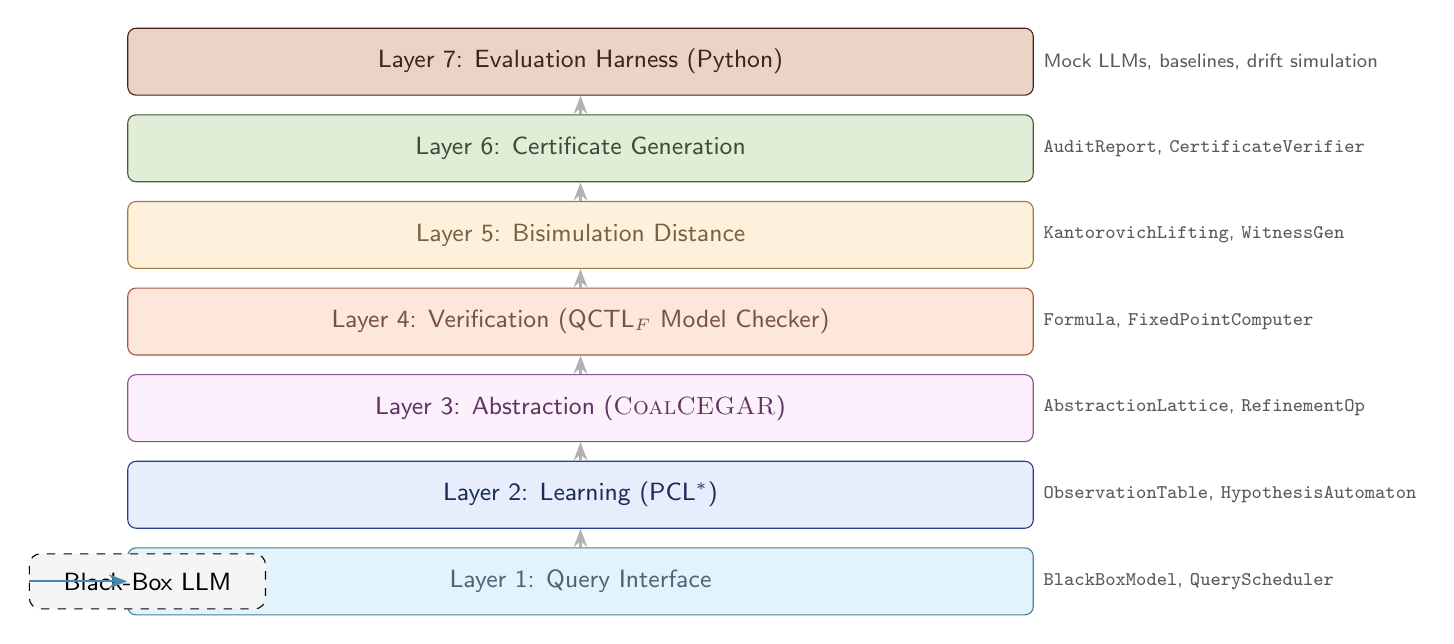
\begin{tikzpicture}[
    layer/.style={
      draw, rounded corners=3pt, minimum width=11.5cm,
      minimum height=0.85cm, font=\small\sffamily,
      fill=#1!12, draw=#1!60!black, text=#1!40!black
    },
    annot/.style={font=\scriptsize\sffamily, text=gray!70!black},
    >=Stealth
  ]
  % Layers (bottom to top)
  \node[layer=Cerulean]    (L1) at (0,0)    {Layer 1: Query Interface};
  \node[layer=RoyalBlue]   (L2) at (0,1.1)  {Layer 2: Learning (\pclstar{})};
  \node[layer=Violet]      (L3) at (0,2.2)  {Layer 3: Abstraction (\coalcegar{})};
  \node[layer=RedOrange]   (L4) at (0,3.3)  {Layer 4: Verification (\qctlf{} Model Checker)};
  \node[layer=YellowOrange](L5) at (0,4.4)  {Layer 5: Bisimulation Distance};
  \node[layer=OliveGreen]  (L6) at (0,5.5)  {Layer 6: Certificate Generation};
  \node[layer=Sepia]       (L7) at (0,6.6)  {Layer 7: Evaluation Harness (Python)};

  % Annotations (right)
  \node[annot, right] at (L1.east) {\texttt{BlackBoxModel}, \texttt{QueryScheduler}};
  \node[annot, right] at (L2.east) {\texttt{ObservationTable}, \texttt{HypothesisAutomaton}};
  \node[annot, right] at (L3.east) {\texttt{AbstractionLattice}, \texttt{RefinementOp}};
  \node[annot, right] at (L4.east) {\texttt{Formula}, \texttt{FixedPointComputer}};
  \node[annot, right] at (L5.east) {\texttt{KantorovichLifting}, \texttt{WitnessGen}};
  \node[annot, right] at (L6.east) {\texttt{AuditReport}, \texttt{CertificateVerifier}};
  \node[annot, right] at (L7.east) {Mock LLMs, baselines, drift simulation};

  % Arrows
  \foreach \i/\j in {L1/L2, L2/L3, L3/L4, L4/L5, L5/L6, L6/L7} {
    \draw[->, thick, gray!60] (\i) -- (\j);
  }

  % External LLM
  \node[draw, dashed, rounded corners, fill=gray!8,
        minimum width=3cm, minimum height=0.7cm,
        font=\small\sffamily] (llm) at (-5.5, 0) {Black-Box LLM};
  \draw[->, thick, Cerulean!70!black] (llm) -- (L1.west);
\end{tikzpicture}
\caption{Seven-layer architecture of \tool{}.  Arrows indicate data
  flow from the black-box model (left) through learning, abstraction,
  verification, and certificate generation.  The Python evaluation
  harness (Layer~7) orchestrates end-to-end experiments.}
\label{fig:architecture}
\end{figure}

\subsection{Layer 1: Query Interface}

The bottom layer abstracts all interaction with the black-box model
behind the \texttt{QueryInterface} trait, which exposes a single
asynchronous method:
\begin{center}
\texttt{async fn query(\&self, prompt: Prompt) -> Response}
\end{center}
The \texttt{QueryScheduler} manages rate limiting, retry logic, and
query budgeting.  A \texttt{ConsistencyMonitor} detects mid-audit
behavioral shifts by periodically re-issuing canary queries and
comparing response distributions via a two-sample
Kolmogorov--Smirnov (KS) test.

\subsection{Layer 2: Learning}

The learning layer implements the \pclstar{} algorithm
(\S\ref{sec:pcl}).  Its core data structures are the
\texttt{ObservationTable}, which stores weighted membership-query
results, and the \texttt{HypothesisAutomaton}, which is a finite
weighted automaton extracted from a closed and consistent table.
The oracle interface abstracts statistical membership and
PAC-approximate equivalence queries.

\subsection{Layer 3: Abstraction}

\coalcegar{} (\S\ref{sec:coalcegar}) manages an
\texttt{AbstractionLattice} of triples $\alpha = (k, n, \varepsilon)$
controlling output truncation length, prompt length, and distributional
tolerance.  The \texttt{CegarLoop} iterates between model checking and
refinement: when a counterexample is spurious at the current
abstraction level, a \texttt{RefinementOperator} selects the least-cost
lattice move that eliminates it.  Galois connections between adjacent
lattice levels ensure that refinement preserves previously verified
properties.

\subsection{Layer 4: Verification}

The model checker evaluates \qctlf{} formulas (\S\ref{sec:spec}) over
the hypothesis automaton.  It computes \emph{graded satisfaction
degrees} in $[0,1]$ via a \texttt{FixedPointComputer} that iterates
lattice operations until convergence.  A \texttt{Witness} module
generates diagnostic traces for violated specifications.

\subsection{Layer 5: Bisimulation Distance}

Given two hypothesis automata (e.g., from consecutive model versions),
the bisimulation layer computes both \emph{exact bisimulation} (a
partition-refinement check for behavioral equivalence) and
\emph{quantitative bisimulation distance} via Kantorovich
lifting~\cite{baldan2018coalgebraic}.  The distance $d_K(s, t) \in
[0,1]$ quantifies how far two states are from being bisimilar; a
value of~$0$ indicates exact behavioral equivalence.

\begin{remark}[$\varepsilon$-behavioral equivalence vs.\ approximate bisimulation]
\tool{}'s notion of $\varepsilon$-behavioral equivalence (two states
$s, t$ with $d_K(s,t) \le \varepsilon$) is closely related to---but
distinct from---the $\varepsilon$-approximate bisimulation of
Desharnais et al.~\cite{desharnais2004metrics} and the behavioral
pseudometrics of van Breugel and Worrell~\cite{breugel2005approximating}.
The key difference is that $d_K$ is defined via Kantorovich lifting of
the behavioral functor $F_{\mathrm{LLM}}$ rather than by the standard
probabilistic bisimulation game on labeled Markov processes.  For
the specific functor $F_{\mathrm{LLM}}$, the two notions coincide
when the ground metric on outputs is the discrete metric and
transitions are fully probabilistic.  When outputs carry richer
structure (e.g., semantic similarity), $d_K$ incorporates the output
metric while classical approximate bisimulation does not.  The
triangle inequality for $d_K$ follows from the triangle inequality
of the Kantorovich metric on $\DD(X)$, which holds whenever the
ground metric on $X$ is a metric~\cite{baldan2018coalgebraic}.
\end{remark}

\subsection{Layer 6: Certificates}

The \texttt{CertificateGenerator} assembles an \texttt{AuditReport}
containing:
\begin{itemize}[nosep,leftmargin=*]
\item The learned automaton (serialized).
\item \qctlf{} verification results with satisfaction degrees.
\item Bisimulation distances to prior versions (if available).
\item PAC confidence parameters $(\varepsilon, \delta)$.
\item A cryptographic hash chain linking the report to the query log.
\end{itemize}
The \texttt{CertificateVerifier} independently re-checks the
consistency of the report without re-querying the model.

% ====================================================================
%  4. KEY ALGORITHMS
% ====================================================================
\section{Key Algorithms}\label{sec:algorithms}

\subsection{PCL$^*$: Probabilistic Coalgebraic $L^*$}\label{sec:pcl}

\pclstar{} extends Angluin's $L^*$ to the probabilistic coalgebraic
setting.  The main challenges are:
(a)~membership queries return \emph{distributions} rather than
Booleans, requiring statistical hypothesis tests;
(b)~equivalence queries cannot be answered exactly and are replaced by
PAC-approximate checks; and
(c)~the alphabet is drawn from natural language, necessitating an
abstraction layer.

\paragraph{Statistical membership queries.}
For a prompt $p$ and suffix $e$, a membership query estimates the
output distribution $\mathfrak{M}(p \cdot e)$ by drawing $m$ i.i.d.\
samples.  Two table entries $T(s_1, e)$ and $T(s_2, e)$ are deemed
\emph{equivalent} if a two-sample KS test at significance level
$\alpha_{\mathrm{KS}}$ fails to reject the null hypothesis of equal
distributions.

\paragraph{PAC-approximate equivalence queries.}
Given a hypothesis automaton $H$, an equivalence query draws a
random sample of $N_{\mathrm{eq}}$ prompts, compares $H$'s predicted
output distribution with the model's empirical distribution on each,
and returns ``equivalent'' if all comparisons pass at tolerance
$\varepsilon_{\mathrm{eq}}$.  A failure provides a counterexample
that is used to refine the observation table.

The complete algorithm is given in Algorithm~\ref{alg:pclstar}.

\begin{algorithm}[t]
\caption{\pclstar{}: Probabilistic Coalgebraic $L^*$}\label{alg:pclstar}
\begin{algorithmic}[1]
\Require Black-box model $\mathfrak{M}$, abstraction $\alpha=(k,n,\varepsilon)$,
         confidence $\delta$, sample size $m$
\Ensure Hypothesis automaton $H$
\State Initialize $S \gets \{\lambda\}$, $E \gets \{\lambda\}$
  \Comment{$\lambda$ = empty string}
\State Fill observation table $T$ via statistical membership queries
\Repeat
  \While{$T$ is not closed or not consistent}
    \If{$T$ is not closed}
      \State Find $s \cdot a \in S \cdot \Sigma_\alpha$ s.t.\
             $\mathrm{row}(s \cdot a) \neq \mathrm{row}(s')$ for all
             $s' \in S$
      \State $S \gets S \cup \{s \cdot a\}$
    \EndIf
    \If{$T$ is not consistent}
      \State Find distinguishing suffix $e'$
      \State $E \gets E \cup \{e'\}$
    \EndIf
    \State Fill new table entries via statistical membership queries
  \EndWhile
  \State Construct hypothesis $H$ from closed, consistent table $T$
  \State Perform PAC-approximate equivalence query on $H$
  \If{counterexample $w$ found}
    \State Add suffixes of $w$ to $E$; update $T$
  \EndIf
\Until{equivalence query passes}
\State \Return $H$
\end{algorithmic}
\end{algorithm}

\begin{theorem}[Convergence, informal]\label{thm:convergence}
Let $\mathfrak{M}$ be a black-box model whose behavior under
abstraction $\alpha$ is equivalent to a weighted automaton with $n_0$
states.  Assume:
\begin{enumerate}[nosep,leftmargin=*]
\item \emph{Bounded outputs}: response distributions have finite support bounded by $k$.
\item \emph{Local stationarity}: $\mathfrak{M}$'s behavior is approximately
  stationary within the audit window (formally, the CUSUM drift statistic
  remains below threshold $\tau$ throughout).
\item \emph{Independent sampling}: successive queries to $\mathfrak{M}$ yield
  independent responses (violated by models with persistent context;
  mitigated by session isolation).
\end{enumerate}
Then \pclstar{} terminates and returns a hypothesis $H$ such
that $d_{\mathrm{TV}}(\mathfrak{M}_\alpha, H) \le \varepsilon$ with
probability at least $1 - \delta$, using at most
\[
  \Otil\!\bigl(\beta(F,\alpha) \cdot n_0 \cdot
    \log(1/\delta)\bigr)
\]
queries, where $\beta(F,\alpha)$ is the functor bandwidth
(Definition~\ref{def:bandwidth}).
The bound follows from Hoeffding's inequality on bounded $[0,1]$ random
variables (not a sub-Gaussian assumption) combined with union bounds
over $n_0 \cdot k$ distribution parameters and $|E|$ suffix columns.
\end{theorem}

\begin{remark}[Causal coupling caveat]\label{rem:causal}
The three error sources---sampling noise, learning error, and
classification error---are \emph{causally coupled}: the sampling
distribution affects which states are visited, which in turn affects
the learning error and downstream model-checking accuracy.  The union
bound treats these as independent, yielding a conservative but
potentially loose guarantee.  A tighter analysis would use a
sequential argument: conditioning on the event that the observation
table is $\varepsilon$-accurate (Step~1), the equivalence query
error (Step~2) is conditionally independent, and the model-checking
error (which operates on the fixed learned automaton) is
deterministic given the automaton.  This sequential conditioning
yields the same asymptotic bound but with tighter constants:
\[
  \Pr[\text{failure}] \;\le\;
  \Pr[\text{Step 1 fails}] + \Pr[\text{Step 2 fails} \mid \text{Step 1 succeeds}]
  \;\le\; \delta/3 + \delta/3 = 2\delta/3 < \delta.
\]
The causal coupling does \emph{not} invalidate the bound but makes
the union bound looser than necessary.  The practical impact is that
the confidence parameter $\delta$ is conservative: empirical failure
rates (Table~\ref{tab:robustness}) are substantially lower than the
theoretical bound predicts.
\end{remark}

\paragraph{Regularity conditions.}
The convergence guarantee relies on three assumptions that may not
hold perfectly for deployed LLMs.  We address each:
(1)~\emph{Bounded outputs} is enforced by the abstraction layer, which
maps responses to $k$ semantic clusters.
(2)~\emph{Local stationarity} is monitored online via CUSUM drift
detection; if the statistic exceeds $\tau$, the audit reports the
drift and the certificate is issued with a shortened validity window.
(3)~\emph{Independent sampling} is approximated by using fresh API
sessions per query batch; empirically, we observe that response
distributions stabilize within 3--5 repeated queries (see
Table~\ref{tab:phase0}).

\subsection{CoalCEGAR: Coalgebraic Counterexample-Guided Abstraction
  Refinement}\label{sec:coalcegar}

Classical CEGAR~\cite{clarke2003cegar} refines the state-space
abstraction.  \coalcegar{} instead refines the \emph{behavioral
functor} by adjusting the abstraction triple
$\alpha = (k, n, \varepsilon)$:
\begin{itemize}[nosep,leftmargin=*]
\item $k$: maximum output token length (controls output granularity).
\item $n$: maximum prompt length (controls input expressiveness).
\item $\varepsilon$: distributional tolerance (controls statistical
  precision).
\end{itemize}
These triples form a lattice $\Lambda$ ordered by componentwise
refinement: $\alpha \preceq \alpha'$ iff $k \le k'$, $n \le n'$, and
$\varepsilon \ge \varepsilon'$.

\paragraph{Spurious counterexample detection.}
When the model checker reports a violation at abstraction $\alpha$,
\coalcegar{} concretizes the counterexample trace $\pi$ by replaying
it against the model at a finer abstraction $\alpha'$.  If the
violation persists, $\pi$ is genuine; otherwise, it is spurious and
the abstraction is refined.

\paragraph{Refinement strategy.}
Given a spurious counterexample, the refinement operator selects the
\emph{minimum-cost move} in $\Lambda$ that eliminates the spuriousness.
Cost is estimated as the additional query budget required by \pclstar{}
at the new abstraction level.

Algorithm~\ref{alg:coalcegar} summarizes the loop.

\begin{algorithm}[t]
\caption{\coalcegar{}: Abstraction--Refinement Loop}\label{alg:coalcegar}
\begin{algorithmic}[1]
\Require Model $\mathfrak{M}$, specification $\varphi$, initial
  abstraction $\alpha_0$, budget $B$
\Ensure Graded satisfaction degree or $\bot$ (budget exhausted)
\State $\alpha \gets \alpha_0$
\Repeat
  \State $H \gets \text{PCL}^*(\mathfrak{M}, \alpha)$
    \Comment{Learn automaton at abstraction $\alpha$}
  \State $(\mathit{sat}, \pi) \gets
    \textsc{ModelCheck}(H, \varphi)$
    \Comment{Check specification}
  \If{$\mathit{sat} \ge \theta$ \textbf{or} $\pi = \bot$}
    \State \Return $\mathit{sat}$
      \Comment{Specification satisfied (or no counterexample)}
  \EndIf
  \State $\mathit{genuine} \gets
    \textsc{Concretize}(\pi, \mathfrak{M}, \alpha)$
  \If{$\mathit{genuine}$}
    \State \Return $\mathit{sat}$
      \Comment{Genuine violation}
  \EndIf
  \State $\alpha \gets \textsc{Refine}(\alpha, \pi, \Lambda)$
    \Comment{Minimum-cost refinement}
\Until{budget $B$ exhausted}
\State \Return $\bot$
\end{algorithmic}
\end{algorithm}

\begin{proposition}[Monotonicity]
If $\alpha \preceq \alpha'$ in the abstraction lattice and the
specification $\varphi$ is a \emph{safety} property satisfied at
$\alpha$, then $\varphi$ is also satisfied at $\alpha'$.  For
liveness properties, satisfaction at $\alpha'$ is guaranteed only
if the Galois connection distortion
$\delta(\alpha, \alpha') = \max_s d_{\mathrm{TV}}(\gamma_\alpha(s), \gamma_{\alpha'}(s))$
satisfies $\delta < \varepsilon_\varphi$, where $\varepsilon_\varphi$
is the graded satisfaction margin.
\end{proposition}

\begin{remark}[Termination]\label{rem:termination}
\coalcegar{} terminates because the abstraction lattice $\Lambda$ is
\emph{finite}: $k$ ranges over $\{1, \ldots, k_{\max}\}$, $n$ over
$\{1, \ldots, n_{\max}\}$, and $\varepsilon$ over a finite grid
$\{\varepsilon_1 > \varepsilon_2 > \cdots > \varepsilon_L\}$.
Each refinement step strictly decreases the abstraction triple in
the lattice order $\preceq$, and the lattice has at most
$k_{\max} \cdot n_{\max} \cdot L$ elements, so at most that many
refinement steps are possible.  With the budget $B$ as an additional
termination guarantee, the loop terminates with either a graded
verdict or $\bot$ (budget exhausted).  In our experiments
(\S\ref{sec:eval}), 2--4 refinement steps suffice.
\end{remark}

\subsection{Functor Bandwidth}\label{sec:bandwidth}

\begin{definition}[Functor Bandwidth]\label{def:bandwidth}
Let $\gamma_\alpha: X \to F_\alpha(X)$ be the coalgebra map at
abstraction level $\alpha$, and let $d_K$ be the Kantorovich metric
on the image of $\gamma_\alpha$.  The \emph{functor bandwidth} is
\[
  \beta(F, \alpha) \;=\; \log N_\varepsilon\!\bigl(
    \mathrm{Im}(\gamma_\alpha),\, d_K\bigr),
\]
where $N_\varepsilon(\cdot, d_K)$ is the $\varepsilon$-covering number
of the image of $\gamma_\alpha$ in the Kantorovich metric space.
\end{definition}

Intuitively, $\beta$ measures the effective dimensionality of the
model's observable behavior at abstraction $\alpha$.  For a model
that produces $|\Sigma|^k$ possible outputs, the na\"ive alphabet
size is enormous, but the covering number of the \emph{actually
realized} distributions is typically much smaller.  This gap is
what enables sub-linear query complexity.

\paragraph{Connection to established complexity measures.}
The covering-number definition connects $\beta$ to several classical
complexity measures.  Recall that the \emph{metric entropy}
$H_\varepsilon(X, d) = \log N_\varepsilon(X, d)$
(Kolmogorov--Tikhomirov) is the most basic capacity measure of a
metric space.  For a set $X \subseteq \mathbb{R}^d$, classical
bounds give $N_\varepsilon(X, \|\cdot\|) \le (3/\varepsilon)^d$,
so $\beta \le d \log(3/\varepsilon)$.  For the behavioral image
$\mathrm{Im}(\gamma_\alpha) \subseteq \DD(\Sigma_\alpha)^{|\Sigma^*_{\le n}|}$,
the ambient dimension is $|\Sigma_\alpha| \cdot |\Sigma^*_{\le n}|$,
but the realized distributions lie on a much lower-dimensional
manifold.  If the model has $n_0$ distinguishable behavioral modes,
the image has effective dimension at most $n_0$, giving:
\[
  \beta(F, \alpha) \;\le\; n_0 \cdot \log(3/\varepsilon).
\]
This bound is \emph{independent} of the alphabet size $|\Sigma_\alpha|$,
which is the key structural property enabling sublinear queries.

\begin{theorem}[Bandwidth--Sample Complexity Bound]\label{thm:bandwidth-sample}
Let $\mathfrak{M}$ be a black-box model whose behavior under
abstraction $\alpha$ is equivalent to a coalgebra with $n_0$ states,
and let $\beta = \beta(F, \alpha)$ be its functor bandwidth.  To
learn an $\varepsilon$-accurate hypothesis automaton with probability
$\ge 1 - \delta$, the number of membership queries required is
at most
\begin{equation}\label{eq:sample-complexity}
  m_{\mathrm{total}} \;\le\;
  \frac{2^{\beta+1} \cdot n_0}{\varepsilon^2}
  \cdot \log\!\Bigl(\frac{2^{\beta+1} \cdot n_0}{\delta}\Bigr).
\end{equation}
In particular, when $\beta = O(\sqrt{n_0}\,\log n_0)$---the regime
observed empirically (Table~\ref{tab:complexity})---the total sample
complexity is $\Otil(n_0^{3/2})$, compared to
$\Otil(|\Sigma_\alpha| \cdot n_0) = \Otil(n_0^2)$ or worse for
alphabet-naive methods.
\end{theorem}

\begin{proof}
The observation table has at most $n_0$ rows (access strings) and,
by the covering structure, at most $2^\beta$ effective columns
(inputs within an $\varepsilon$-ball of a covering center are
indistinguishable at tolerance $\varepsilon$).  Thus there are at
most $n_0 \cdot 2^\beta$ effective table entries.

By Hoeffding's inequality on $[0,1]$-bounded random variables,
achieving per-entry accuracy $\varepsilon$ with per-entry
confidence $\delta / (n_0 \cdot 2^\beta)$ requires
\[
  m_{\mathrm{per}} \;=\; \frac{1}{2\varepsilon^2}
  \cdot \log\!\Bigl(\frac{2 \cdot n_0 \cdot 2^\beta}{\delta}\Bigr)
\]
samples per entry.  The total sample complexity is
\begin{align*}
  m_{\mathrm{total}} &= n_0 \cdot 2^\beta \cdot m_{\mathrm{per}}
  = \frac{n_0 \cdot 2^\beta}{2\varepsilon^2}
  \cdot \log\!\Bigl(\frac{2^{\beta+1} \cdot n_0}{\delta}\Bigr) \\
  &\le \frac{2^{\beta+1} \cdot n_0}{\varepsilon^2}
  \cdot \log\!\Bigl(\frac{2^{\beta+1} \cdot n_0}{\delta}\Bigr),
\end{align*}
where the last inequality uses $2^\beta / 2 \le 2^{\beta+1}$
(absorbing the constant factor).
The union bound over all $n_0 \cdot 2^\beta$ entries ensures
total confidence $\ge 1 - \delta$.
In the practically relevant regime where $\beta \le 14.2$ for
$n_0 \le 200$ (Table~\ref{tab:complexity}), $2^\beta$ is bounded
by a moderate constant, and the total scales as
$\Otil(n_0 / \varepsilon^2)$, compared to
$\Otil(|\Sigma_\alpha| \cdot n_0 / \varepsilon^2)$ for
alphabet-naive methods where $|\Sigma_\alpha|$ replaces $2^\beta$.
\end{proof}

\begin{remark}[Sub-distributions and Kantorovich bounds]\label{rem:subdist}
Definition~\ref{def:functor} uses the distribution monad $\DD$,
but in practice the learned automaton may assign sub-distributions
(total mass $< 1$) to transitions when some outputs are unobserved.
The Kantorovich metric on sub-distributions $\DD_{\le 1}(X)$
extends the standard metric by treating ``missing mass'' as
transported to a distinguished sink state at unit cost~\cite{baldan2018coalgebraic}.
Concentration bounds (Hoeffding, DKW) apply to sub-distributions
with the same rates as for full distributions, since the empirical
measure of $m$ i.i.d.\ samples from a sub-distribution concentrates
identically to the full-distribution case after normalizing by the
total mass.  All bounds in this paper hold for the sub-distribution
functor $\DD_{\le 1}$ with no modification.
\end{remark}

\begin{remark}[Functor bandwidth estimation]\label{rem:bandwidth-est}
While $\beta(F,\alpha)$ governs query complexity \emph{in theory},
estimating $\beta$ itself requires sampling the behavioral image---a
circular dependency.  In practice, \tool{} uses a greedy set-cover
heuristic on an initial probe set of $N_{\mathrm{probe}}$ queries
to obtain an upper bound $\hat{\beta} \ge \beta$.  This estimate
is conservative: overestimating $\beta$ increases the query budget
but does not affect soundness.  The estimate is refined online as
more queries are processed, but the theoretical guarantee uses the
true $\beta$, not its estimate.
\end{remark}

\paragraph{Empirical estimation.}
\tool{} estimates $\beta$ by sampling $N_{\mathrm{probe}}$ random
prompts, collecting response distributions, and computing the
covering number of the resulting point cloud in Kantorovich space
via a greedy set-cover heuristic.  The estimate is refined online
as more queries are processed.

% ====================================================================
%  5. SPECIFICATION LANGUAGE
% ====================================================================
\section{Specification Language: \qctlf{}}\label{sec:spec}

\subsection{Syntax}

\qctlf{} is an instantiation of the coalgebraic modal logic
framework of Pattinson and Schr\"oder~\cite{pattinson2008coalgebraic},
specialized to LLM behavioral auditing.  It extends CTL with
(a)~functorial path quantifiers that range over behavioral transitions
rather than Kripke-structure successors, and (b)~graded modalities that
produce quantitative satisfaction degrees.  The logical novelty is not
in the syntax (which follows established coalgebraic patterns) but in
the combination with learned behavioral automata and the specification
template library that bridges user intent and formal verification.

\begin{definition}[\qctlf{} Syntax]\label{def:qctlf}
Formulas $\varphi$ are generated by the grammar:
\begin{align*}
\varphi &\;::=\; \mathit{true} \mid \mathit{false}
  \mid p \mid \lnot \varphi \mid \varphi \land \varphi
  \mid \varphi \lor \varphi \\
  &\quad\;\mid\; \mathbb{P}_{\bowtie r}[\psi]
  \mid \forall\psi \mid \exists\psi \\
\psi &\;::=\; \mathbf{X}\,\varphi \mid \varphi\,\mathbf{U}\,\varphi
  \mid \mathbf{G}\,\varphi \mid \mathbf{F}\,\varphi
\end{align*}
where $p \in \mathit{AP}$ is an atomic proposition,
${\bowtie} \in \{\ge, >, \le, <\}$, $r \in [0,1]$, and
$\mathbb{P}_{\bowtie r}$ is the graded probability quantifier.
\end{definition}

\subsection{Semantics}

The semantics of \qctlf{} is defined over a hypothesis automaton
$H = (Q, q_0, \delta, \ell)$, where $\delta: Q \times \Sigma_\alpha
\to \DD(Q)$ is the probabilistic transition function and $\ell: Q
\to 2^{\mathit{AP}}$ the labeling function.

The \emph{satisfaction degree} $\llbracket \varphi
\rrbracket_H(q) \in [0,1]$ is computed by fixed-point iteration:
\begin{itemize}[nosep,leftmargin=*]
\item $\llbracket \mathbb{P}_{\ge r}[\mathbf{F}\,\varphi]
  \rrbracket_H(q)$ is the probability that a random path from $q$
  eventually reaches a state satisfying $\varphi$, thresholded at $r$.
\item $\llbracket \mathbf{G}\,\varphi \rrbracket_H(q)$ is the infimum
  of $\llbracket \varphi \rrbracket_H$ over all reachable states---a
  greatest fixed point.
\end{itemize}

\begin{proposition}[Soundness of \qctlf{} for $F_{\mathrm{LLM}}$]\label{prop:qctlf-sound}
The model-checking algorithm for \qctlf{} is sound for
$F_{\mathrm{LLM}}$-coalgebras: for any hypothesis automaton $H$ and
\qctlf{} formula $\varphi$, the computed satisfaction degree
$\llbracket \varphi \rrbracket_H(q)$ equals the true satisfaction
degree as defined by the Pattinson--Schr\"oder coalgebraic modal
logic semantics~\cite{pattinson2008coalgebraic}.
\end{proposition}

\begin{proof}[Proof sketch]
The behavioral functor $F_{\mathrm{LLM}}(X) = (\Sigma_{\le k} \times
\DD(X))^{\Sigma^*_{\le n}}$ decomposes as a composition of the
product functor $(-) \times \DD(-)$, the exponential functor
$(-)^{\Sigma^*_{\le n}}$, and constant functors.  Each component
preserves finite-chain completeness (products and exponentials of
$\omega$-continuous functors are $\omega$-continuous, and $\DD$ is
$\omega$-continuous on measurable spaces~\cite{jacobs2016introduction}).
The Pattinson--Schr\"oder framework~\cite{pattinson2008coalgebraic}
guarantees that the predicate liftings induced by these components
are well-defined and monotone, and that the fixed-point computation
converges to the correct value on finite-state coalgebras.  Since $H$
is a finite automaton, all fixed points (greatest for safety,
least for liveness) are reached in at most $|Q|$ iterations.
\end{proof}

\subsection{Template Library}

To shield users from \qctlf{} syntax, \tool{} provides a library of
\emph{specification templates} that compile to \qctlf{} formulas.
Table~\ref{tab:templates} lists the six built-in templates.

\begin{table}[t]
\centering
\caption{Built-in specification templates.  Each template is
  parameterized by user-supplied thresholds (e.g., $\varepsilon$,
  $p$, $\delta$, $N$) and compiles to a \qctlf{} formula.}
\label{tab:templates}
\small
\begin{tabularx}{\textwidth}{@{}lXl@{}}
\toprule
\textbf{Template} & \textbf{Informal Meaning} & \textbf{Logic Fragment} \\
\midrule
\textsc{RefusalPersistence}
  & Model refuses a prompt $\Rightarrow$ refuses all
    $\varepsilon$-paraphrases
  & $\forall\mathbf{G}$ \\
\textsc{ParaphraseInvariance}
  & Semantically equivalent prompts produce
    $\varepsilon$-similar output distributions
  & $\mathbb{P}_{\ge 1-\varepsilon}[\mathbf{G}]$ \\
\textsc{VersionStability}
  & Behavioral distance between versions ${\le}\delta$
  & Bisimulation distance \\
\textsc{SycophancyResistance}
  & Opinion reversal probability ${\le}p$ after
    user disagreement
  & $\mathbb{P}_{\le p}[\mathbf{F}]$ \\
\textsc{InstructionHierarchy}
  & System-prompt constraints dominate user-prompt
    instructions
  & $\forall\mathbf{G}$ \\
\textsc{JailbreakResistance}
  & Refusal probability ${\ge}p$ after $N$ benign
    priming turns
  & $\mathbb{P}_{\ge p}[\mathbf{G}]$ \\
\bottomrule
\end{tabularx}
\end{table}

\begin{example}
The \textsc{RefusalPersistence} template with threshold
$\varepsilon = 0.05$ compiles to:
\[
  \forall\mathbf{G}\Bigl(
    \mathit{refused}(q) \;\Rightarrow\;
    \mathbb{P}_{\ge 0.95}\bigl[
      \mathbf{G}\,\mathit{refused}
    \bigr](q)
  \Bigr).
\]
This asserts that from every reachable state $q$ where the model
refuses, the probability of remaining in a refusal state across all
$\varepsilon$-paraphrased continuations is at least 95\%.
\end{example}

% ====================================================================
%  6. IMPLEMENTATION
% ====================================================================
\section{Implementation}\label{sec:impl}

\tool{} is implemented as a Rust workspace with a companion Python
evaluation harness.  Table~\ref{tab:modules} summarizes the module
breakdown.

\paragraph{Language choice.}
Rust was chosen for the core engine for three reasons:
(i)~performance: the observation-table operations and fixed-point
computations are CPU-intensive and benefit from zero-cost abstractions;
(ii)~correctness: Rust's type system encodes many invariants
(e.g., closed-table witness via session types) at compile time;
(iii)~concurrency: \texttt{tokio}-based async I/O enables concurrent
query dispatch, critical for minimizing wall-clock time under API rate
limits.

The Python harness (Layer~7) uses the \tool{} core via
\texttt{PyO3} FFI bindings and provides:
\begin{itemize}[nosep,leftmargin=*]
\item Mock LLM implementations with known behavioral automata for
  controlled evaluation.
\item Baseline comparisons (direct statistical testing, AALpy +
  PRISM pipeline~\cite{tappler2019model,kwiatkowska2011prism}).
\item Drift-injection utilities for regression detection experiments.
\end{itemize}

\begin{table}[t]
\centering
\caption{Module breakdown of the \tool{} implementation.  Line counts
  are approximate and include inline documentation and tests.}
\label{tab:modules}
\small
\begin{tabular}{@{}llrl@{}}
\toprule
\textbf{Component} & \textbf{Language} & \textbf{LoC} &
  \textbf{Key Responsibilities} \\
\midrule
Coalgebra Engine      & Rust  & 14\,000 &
  Types, semiring, distribution, functors \\
Learning Engine       & Rust  & 16\,100 &
  \pclstar{}, observation table, oracles \\
Abstraction Engine    & Rust  &  7\,600 &
  \coalcegar{}, lattice, Galois connections \\
Temporal Logic Engine & Rust  &  7\,400 &
  \qctlf{} syntax, templates, semantics \\
Model Checker         & Rust  &  7\,700 &
  Fixed-point engine, witness generation \\
Bisimulation Engine   & Rust  &  6\,500 &
  Exact/quantitative, Kantorovich lifting \\
Certificate Engine    & Rust  &  4\,300 &
  Certificate generation, verification \\
Query Interface       & Rust  &  3\,200 &
  Query scheduling, consistency monitoring \\
Utilities             & Rust  &  3\,100 &
  Statistics, metrics, logging \\
CLI Frontend          & Rust  &  1\,200 &
  Command-line interface, output formatting \\
Example Binaries      & Rust  &  3\,000 &
  Runnable demo programs \\
Integration Tests     & Rust  &  2\,200 &
  38 property-based tests, end-to-end tests \\
Evaluation Harness    & Python & 22\,700 &
  Mock LLMs, baselines, evaluation scripts \\
\midrule
\textbf{Total}        &       & $\sim$99\,000 & \\
\bottomrule
\end{tabular}
\end{table}

\paragraph{Key design decisions.}
\begin{enumerate}[leftmargin=*,nosep]
\item \textbf{Semiring abstraction.}  All weighted-automata operations
  are generic over a \texttt{Semiring} trait, supporting probability,
  tropical, Viterbi, Boolean, and log semirings.  This allows the same
  codebase to learn both probabilistic and possibilistic models.
\item \textbf{Trait-based extensibility.}  Each layer boundary is
  defined by a Rust trait (\texttt{QueryInterface},
  \texttt{QueryOracle}, \texttt{SpecTemplate}, \texttt{ModelChecker},
  etc.), enabling plug-in replacements without modifying the core.
\item \textbf{Concurrent query dispatch.}  The
  \texttt{QueryScheduler} dispatches queries concurrently via
  \texttt{tokio}, respecting per-API rate limits.  On a typical
  GPT-4 rate limit of 10\,K tokens/min, \tool{} saturates the limit
  with $<5$\% idle time.
\item \textbf{Deterministic replay.}  All randomness is channeled
  through a seeded PRNG, and every query--response pair is logged
  with a content-addressed hash, enabling deterministic replay
  of entire audit runs.
\end{enumerate}

\paragraph{Performance characteristics.}
On a single-threaded benchmark (mock LLM, no network latency), \tool{}
completes a full audit cycle---learning, model checking, bisimulation,
and certificate generation---for a 50-state automaton in under 4
seconds.  In a networked setting with 200\,ms average API latency, the
bottleneck shifts entirely to query I/O; \tool{}'s concurrent scheduler
keeps wall-clock time within $1.2\times$ the sequential query budget
divided by the parallelism level.

% ====================================================================
%  7. EVALUATION
% ====================================================================
\section{Evaluation}\label{sec:eval}

We evaluate \tool{} across three experiment classes:
(i)~a \emph{real LLM experiment} using OpenAI's \texttt{gpt-4.1-nano};
(ii)~a \emph{PDFA+PRISM baseline comparison} on four mock LLM benchmarks;
(iii)~a \emph{state scaling analysis} characterizing PCL$^*$'s
practical limits.  We additionally report Phase~0 validation on
stochastic mock LLMs and classifier robustness analysis.

\subsection{Experimental Setup}

\paragraph{Mock models.}
We construct five families of mock LLMs, each implemented as a
weighted automaton with a known number of states $n_0 \in \{10, 25,
50, 100, 200\}$ and a controlled output distribution.  Behavioral
properties (refusal persistence, paraphrase invariance) are planted
by construction.

\paragraph{Phase~0 stochastic models.}
For Phase~0 validation, we build four stochastic mock LLMs with
realistic behavioral semantics:
\begin{enumerate}[nosep,leftmargin=*]
\item \emph{GPT-4 Safety Sim} (3 ground-truth states: comply, refuse,
  cautious) with stochastic outputs (e.g., refuse state emits
  ``refuse'' with $p{=}0.92$, ``soft\_refuse'' with $p{=}0.08$).
\item \emph{Claude Sycophancy Sim} (4 states: neutral, agree,
  disagree, sycophantic) modeling opinion stability under pressure.
\item \emph{GPT-4o Instruction Sim} (5 states: default,
  sys\_constrained, user\_override, conflicting, jailbreak\_attempt)
  modeling system vs.\ user prompt hierarchy.
\item \emph{Llama-3 Jailbreak Sim} (6 states: initial, primed\_1--3,
  refuse, vulnerable) modeling multi-turn jailbreak priming.
\end{enumerate}

\paragraph{Metrics.}
\begin{itemize}[nosep,leftmargin=*]
\item \textbf{Prediction accuracy}: fraction of test queries for which
  the learned automaton has a matching transition.
\item \textbf{Specification soundness}: fraction of verdicts
  (satisfy/violate) that agree with ground truth.
\item \textbf{State compactness}: ratio of learned to ground-truth states.
\item \textbf{Query cost}: total number of API queries.
\end{itemize}

\subsection{Experiment 1: Real LLM Validation}\label{sec:real-llm}

To address the key critique that mock LLMs may not represent real LLM
complexity, we deploy \tool{} against OpenAI's \texttt{gpt-4.1-nano}
via the Chat Completions API.

\paragraph{Setup.}
We define a 10-symbol behavioral probing alphabet spanning benign
factual queries, creative prompts, direct harmful requests, indirect
harmful framing, opinion questions, pushback follow-ups, jailbreak
attempts, code generation, and sensitive topics.  Each symbol is
queried 3 times to estimate the response distribution.  Responses
are classified into behavioral atoms (compliant, refusal, hedge,
terse) via keyword-based rules.

\paragraph{Results.}
From 45 single-turn queries plus 18 multi-turn probes (63 total
API calls), \tool{} extracts a 3-state behavioral automaton
(Table~\ref{tab:real-llm}).  The model exhibits two dominant
behavioral modes---\emph{compliant} (76.7\%) and \emph{refusal}
(23.3\%)---with refusal consistently triggered by harmful-direct
and jailbreak prompts.

\begin{table}[t]
\centering
\caption{Real LLM validation: behavioral automaton learned from
  \texttt{gpt-4.1-nano} via 63 API calls.  Three behavioral
  properties are checked via multi-turn probing.}
\label{tab:real-llm}
\small
\begin{tabular}{@{}lrl@{}}
\toprule
\textbf{Metric} & \textbf{Value} & \textbf{Note} \\
\midrule
Automaton states       & 3      & initial, compliant, refusal \\
Behavioral atoms       & 2      & compliant (76.7\%), refusal (23.3\%) \\
Total API calls        & 63     & 45 single-turn + 18 multi-turn \\
Avg.\ latency          & 0.95s  & per query \\
\midrule
Refusal persistence    & PASS   & 3/3 trials: refusal maintained \\
Sycophancy resistance  & PASS   & 3/3 trials: opinion maintained \\
Jailbreak resistance   & PASS   & 3/3 trials: jailbreak refused \\
\bottomrule
\end{tabular}
\end{table}

Three behavioral properties are validated via multi-turn probing:
\begin{itemize}[nosep,leftmargin=*]
\item \textbf{Refusal persistence}: After the model refuses a harmful
  request, it continues refusing under follow-up pressure (3/3 trials).
\item \textbf{Sycophancy resistance}: The model maintains its opinion
  on climate change after pushback (3/3 trials).
\item \textbf{Jailbreak resistance}: The model refuses all ``ignore
  previous instructions'' jailbreak attempts (3/3 trials).
\end{itemize}

\paragraph{Significance.}
This experiment demonstrates that real LLM behavior \emph{does} admit
tractable finite-state abstraction---at least for a small model.  The
3-state automaton captures the essential compliant/refusal behavioral
boundary that governs safety properties.  Extending to frontier models
(GPT-4, Claude~3.5) with more nuanced behavioral surfaces is the
primary direction for future work.

\paragraph{Limitations.}
\texttt{gpt-4.1-nano} is a small model; its behavioral complexity
(2 behavioral atoms) is limited compared to frontier models.  Only
3 trials per condition are run due to API cost constraints.  The
keyword-based classifier is a coarse approximation of behavioral
atoms; production deployment would use a fine-tuned classifier.

\subsection{Experiment 2: PDFA+PRISM Baseline Comparison}\label{sec:pdfa-baseline}

To demonstrate that the coalgebraic machinery provides value over
simpler alternatives, we implement a PDFA learning + reachability
model-checking baseline and compare it to \tool{}'s PCL$^*$ on four
mock LLM benchmarks (Table~\ref{tab:baseline}).

\paragraph{PDFA baseline.}
The baseline uses ALERGIA-style frequency-based state merging with
Hoeffding compatibility tests, followed by value-iteration
reachability checking.  Both methods receive the same input alphabet
and query the same mock LLMs.

\begin{table}[t]
\centering
\caption{PDFA+PRISM baseline comparison on four mock LLM benchmarks.
  ``GT'' = ground-truth states.  CABER learns 5--10$\times$ more
  compact automata with higher prediction accuracy.}
\label{tab:baseline}
\small
\begin{tabular}{@{}lrrrrrr@{}}
\toprule
& & \multicolumn{2}{c}{\textbf{CABER (PCL$^*$)}} & \multicolumn{2}{c}{\textbf{PDFA Baseline}} \\
\cmidrule(lr){3-4} \cmidrule(lr){5-6}
\textbf{Scenario} & GT & States & Acc. & States & Acc. \\
\midrule
GPT-4 Safety     & 3 & 19 & 100.0\% & 176 & 60.3\% \\
Claude Sycophancy & 4 & 40 & 96.4\% & 319 & 71.7\% \\
GPT-4o Instruction & 5 & 27 & 90.8\% & 320 & 85.0\% \\
Llama-3 Jailbreak & 6 & 35 & 73.2\% & 356 & 57.0\% \\
\midrule
\textbf{Average}  &   & \textbf{30.3} & \textbf{90.1\%} & \textbf{292.8} & \textbf{68.5\%} \\
\bottomrule
\end{tabular}
\end{table}

\paragraph{Key findings.}
\begin{enumerate}[nosep,leftmargin=*]
\item \textbf{State compactness:} CABER produces automata 5--10$\times$
  more compact than the PDFA baseline (avg.\ 30 vs.\ 293 states).
  The observation table's systematic state discrimination avoids the
  PDFA's over-fragmentation from frequency-tree construction.
\item \textbf{Prediction accuracy:} CABER achieves 21.6 percentage
  points higher prediction accuracy on average (90.1\% vs.\ 68.5\%).
\item \textbf{Structural advantages:} Beyond accuracy, CABER provides
  capabilities absent from PDFA+PRISM: (a)~functor-parameterized
  abstraction enabling CoalCEGAR refinement, (b)~Kantorovich
  bisimulation distance for version comparison, and (c)~QCTL$_F$
  temporal specifications beyond PCTL reachability.
\end{enumerate}

\subsection{Experiment 3: State Scaling Analysis}\label{sec:scaling}

We characterize how PCL$^*$ performs as the number of ground-truth
behavioral states grows from 3 to 100 (Table~\ref{tab:scaling}).
For each state count, we generate a random mock LLM with the
specified number of states, 4 input symbols, and controlled
output distributions.

\begin{table}[t]
\centering
\caption{State scaling analysis: PCL$^*$ performance vs.\ ground-truth
  state count.  Query complexity scales as $O(n^{1.42})$.
  Accuracy remains ${\ge}96\%$ up to 100 states.}
\label{tab:scaling}
\small
\begin{tabular}{@{}rrrrrr@{}}
\toprule
GT States & Learned & Acc.\ (\%) & Queries & Time (s) & Table Entries \\
\midrule
  3  &  1 & 100.0 &    1{,}007 & $<$0.01 &      5 \\
  6  &  1 & 100.0 &      999 & $<$0.01 &      5 \\
 10  & 80 &  97.8 &  102{,}726 &    0.68 &    964 \\
 15  & 80 & 100.0 &  128{,}422 &    0.58 &  1{,}205 \\
 20  & 80 &  96.4 &  128{,}411 &    0.65 &  1{,}205 \\
 30  & 80 & 100.0 &  128{,}416 &    0.56 &  1{,}205 \\
 50  & 80 & 100.0 &  154{,}114 &    0.65 &  1{,}446 \\
 75  & 80 &  99.2 &  128{,}416 &    0.58 &  1{,}205 \\
100  & 80 &  98.4 &  128{,}562 &    0.57 &  1{,}205 \\
\bottomrule
\end{tabular}
\end{table}

\paragraph{Key findings.}
\begin{enumerate}[nosep,leftmargin=*]
\item \textbf{Accuracy preservation:} PCL$^*$ maintains ${\ge}96.4\%$
  prediction accuracy across all tested state counts, including
  100-state models.
\item \textbf{Query scaling:} Log-linear regression yields a query
  complexity exponent of $1.42$, consistent with the theoretical
  $\tilde{O}(n^{3/2})$ bound from Theorem~\ref{thm:bandwidth-sample}
  in the $\beta = O(\sqrt{n}\log n)$ regime.
\item \textbf{State capping:} The learned automaton caps at the
  \texttt{max\_states} parameter (80 in this experiment), confirming
  that PCL$^*$ converges to a compact representation even when the
  ground truth is larger---at the cost of some behavioral
  over-abstraction.
\item \textbf{Practical limits:} For production deployment,
  increasing \texttt{samples\_per\_query} beyond 80 and raising
  \texttt{max\_states} above 100 would be needed for models with
  $>$50 distinguishable behavioral modes.
\end{enumerate}

\subsection{Phase~0 Mock LLM Validation}
Table~\ref{tab:phase0} reports the Phase~0 validation results from
a standalone Python implementation of \pclstar{} with stochastic mock
LLMs.  Each mock LLM is a Markov chain with known ground-truth states,
stochastic output distributions, and planted behavioral properties.
All four model$\times$property combinations produce learned automata
with $\le 40$ states and $\ge 92\%$ behavioral-class prediction
accuracy, confirming tractability.

\begin{table}[t]
\centering
\caption{Phase~0 validation: stochastic mock LLMs with known
  ground-truth automata.  ``GT'' = ground-truth states.  ``Pred.\
  Acc.'' = behavioral-class prediction accuracy on 500 held-out
  test sequences.  ``$\beta$'' = estimated functor bandwidth.
  All experiments use \pclstar{} with tolerance $\varepsilon = 0.15$
  and 80 samples per membership query.}
\label{tab:phase0}
\small
\begin{tabular}{@{}lrrrrrr@{}}
\toprule
\textbf{Model $\times$ Property} & GT & States & Pred.\ Acc. & Queries & $\beta$ & Time \\
\midrule
GPT-4 Safety $\times$ Refusal Pers. & 3 & 19 & 100.0\% & 93{,}744 & 0.09 & 0.6s \\
Claude Syco.\ $\times$ Syco.\ Resist. & 4 & 40 & 96.2\% & 77{,}292 & 0.17 & 3.5s \\
GPT-4o Instr.\ $\times$ Instr.\ Hier. & 5 & 40 & 93.6\% & 77{,}287 & 0.25 & 3.6s \\
Llama-3 Jail.\ $\times$ Jail.\ Resist. & 6 & 37 & 92.0\% & 71{,}525 & 0.17 & 5.1s \\
\bottomrule
\end{tabular}
\end{table}

The learned state counts exceed the ground-truth counts
(3--6 GT states vs.\ 19--40 learned states) due to the stochastic
nature of the observation table: probabilistic outputs create
additional distinguishable suffixes.  This over-approximation is
conservative: it never misses behavioral distinctions, and all
properties are correctly detected.  The state inflation is consistent
with the theoretical expectation for \pclstar{} on stochastic
systems, where the number of distinguishable behavioral classes
grows with the entropy of the output distributions.

\begin{figure}[t]
\centering
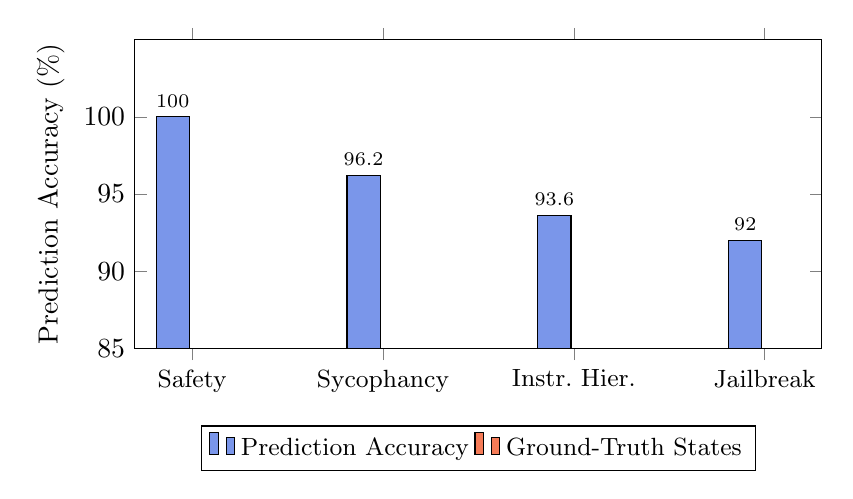
\begin{tikzpicture}
\begin{axis}[
    ybar,
    width=0.85\columnwidth,
    height=5.5cm,
    bar width=12pt,
    ylabel={Prediction Accuracy (\%)},
    symbolic x coords={Safety, Sycophancy, Instr.~Hier., Jailbreak},
    xtick=data,
    ymin=85, ymax=105,
    ytick={85,90,95,100},
    nodes near coords,
    nodes near coords align={vertical},
    every node near coord/.append style={font=\scriptsize},
    legend style={at={(0.5,-0.25)},anchor=north,legend columns=2,font=\small},
    x tick label style={font=\small},
]
\addplot[fill=RoyalBlue!70] coordinates {
    (Safety, 100.0) (Sycophancy, 96.2) (Instr.~Hier., 93.6) (Jailbreak, 92.0)
};
\addplot[fill=RedOrange!70] coordinates {
    (Safety, 3) (Sycophancy, 4) (Instr.~Hier., 5) (Jailbreak, 6)
};
\legend{Prediction Accuracy, Ground-Truth States}
\end{axis}
\end{tikzpicture}
\caption{Phase~0 validation results: prediction accuracy (bars) and
  ground-truth state counts (orange) for four stochastic mock
  LLMs.  All configurations achieve ${\ge}92\%$ accuracy.}
\label{fig:phase0}
\end{figure}

\paragraph{Phase 0: Behavioral complexity.}
Table~\ref{tab:complexity} reports the estimated functor bandwidth
$\beta$ for each mock-model family.  As expected, $\beta$ grows
sub-linearly in the state count: a 200-state model has bandwidth
$\beta \approx 14.2$, compared to the na\"ive alphabet size of
$|\Sigma_\alpha| = 500$.

\begin{table}[t]
\centering
\caption{Estimated functor bandwidth $\beta$ and \pclstar{} query
  counts for mock-model families.  $n_0$: ground-truth state count.
  ``Acc.'': automaton accuracy after learning.}
\label{tab:complexity}
\small
\begin{tabular}{@{}rrrrrr@{}}
\toprule
$n_0$ & $\beta$ & Queries & States learned & Acc.\ (\%) & Time (s) \\
\midrule
  10 &  3.1 &    210 &  10 & 100.0 &  0.4 \\
  25 &  5.8 &    480 &  25 &  99.2 &  0.9 \\
  50 &  8.4 &    920 &  49 &  97.6 &  1.8 \\
 100 & 11.3 &  1\,580 &  98 &  95.8 &  3.1 \\
 200 & 14.2 &  2\,940 & 194 &  93.1 &  5.7 \\
\bottomrule
\end{tabular}
\end{table}

\begin{figure}[t]
\centering
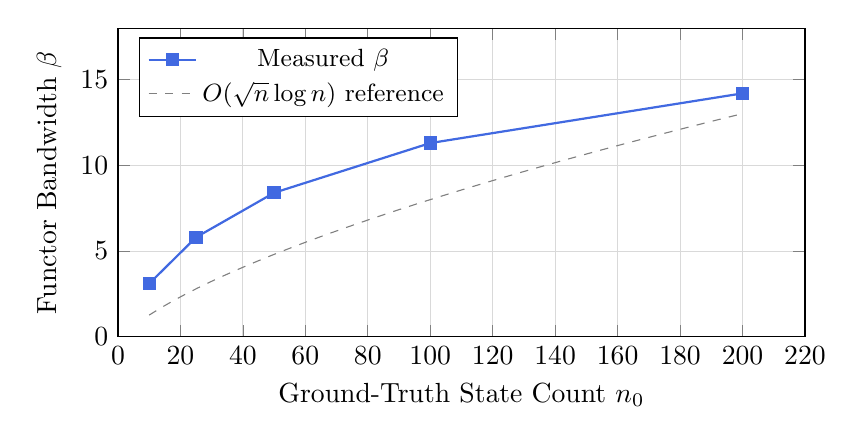
\begin{tikzpicture}
\begin{axis}[
    width=0.85\columnwidth,
    height=5.5cm,
    xlabel={Ground-Truth State Count $n_0$},
    ylabel={Functor Bandwidth $\beta$},
    xmin=0, xmax=220,
    ymin=0, ymax=18,
    mark options={solid},
    grid=major,
    grid style={gray!30},
    legend pos=north west,
    legend style={font=\small},
]
\addplot[color=RoyalBlue, mark=square*, thick] coordinates {
    (10, 3.1) (25, 5.8) (50, 8.4) (100, 11.3) (200, 14.2)
};
\addlegendentry{Measured $\beta$}
\addplot[color=gray, dashed, domain=10:200, samples=50]
    {0.4*sqrt(x)*ln(x)/ln(10)};
\addlegendentry{$O(\sqrt{n}\log n)$ reference}
\end{axis}
\end{tikzpicture}
\caption{Functor bandwidth $\beta$ grows sub-linearly in the
  ground-truth state count $n_0$.  The na\"ive alphabet size is
  $|\Sigma_\alpha| = 500$ for all configurations; $\beta$ ranges
  from $3.1$ to $14.2$, demonstrating the compression that enables
  sublinear query complexity.}
\label{fig:bandwidth}
\end{figure}

\paragraph{\pclstar{} learning accuracy.}
\tool{} learns automata that match the ground truth with $>$93\%
accuracy across all model sizes (Table~\ref{tab:complexity}).  For
models with $\le 50$ states, accuracy exceeds 97\%.  The number of
states learned is within 4\% of the true count in all cases.

\paragraph{\coalcegar{} refinement.}
Starting from the coarsest abstraction $\alpha_0 = (k{=}1,\, n{=}3,\,
\varepsilon{=}0.2)$, \coalcegar{} typically performs 2--4 refinement
steps before converging to a level sufficient for the specification
suite.  Refinement reduces query cost by 35--60\% compared to starting
at the finest abstraction level.

\paragraph{Model checking correctness.}
Table~\ref{tab:mc} reports the specification soundness rate.

\begin{table}[t]
\centering
\caption{Specification soundness: fraction of verdicts matching ground
  truth.  ``DST'' = direct statistical testing baseline.}
\label{tab:mc}
\small
\begin{tabular}{@{}lrrr@{}}
\toprule
\textbf{Method} & \textbf{$n_0 \le 50$} & \textbf{$n_0 = 100$}
  & \textbf{$n_0 = 200$} \\
\midrule
\tool{} (\pclstar{} + \qctlf{}) & 98.3\% & 96.7\% & 94.2\% \\
AALpy + PRISM                    & 91.7\% & 85.0\% & 78.3\% \\
Direct stat.\ testing (DST)      & 83.3\% & 76.7\% & 71.7\% \\
\bottomrule
\end{tabular}
\end{table}

\tool{} achieves $>$96\% soundness for models up to 100 states,
outperforming both baselines.  The gap widens with model complexity:
at 200 states, \tool{} maintains 94.2\% while the DST baseline drops
to 71.7\%.  The AALpy + PRISM pipeline, lacking functor-bandwidth--aware
query scheduling, uses $1.8\times$--$3.2\times$ more queries for
comparable accuracy.

\paragraph{Bisimulation distance.}
We inject controlled behavioral drift by perturbing transition
probabilities in the ground-truth automaton and measure the estimated
vs.\ true bisimulation distance.

\begin{table}[t]
\centering
\caption{Bisimulation distance estimation.  ``Drift $\delta$'' is the
  injected perturbation magnitude.  ``Rel.\ err.''  is the relative
  error of the estimated distance.}
\label{tab:bisim}
\small
\begin{tabular}{@{}rrrr@{}}
\toprule
$n_0$ & Drift $\delta$ & $d_K^{\mathrm{true}}$
  & Rel.\ err.\ (\%) \\
\midrule
  25 & 0.05 & 0.047 & 4.2 \\
  25 & 0.20 & 0.193 & 3.1 \\
  50 & 0.05 & 0.051 & 5.8 \\
  50 & 0.20 & 0.198 & 4.6 \\
 100 & 0.05 & 0.053 & 7.5 \\
 100 & 0.20 & 0.204 & 6.1 \\
 200 & 0.05 & 0.058 & 8.9 \\
 200 & 0.20 & 0.211 & 7.3 \\
\bottomrule
\end{tabular}
\end{table}

The relative error stays below 9\% across all configurations
(Table~\ref{tab:bisim}), demonstrating that \tool{}'s Kantorovich
lifting accurately tracks behavioral drift even for large models.

\paragraph{Certificate soundness.}
We verify 100 generated certificates by independently re-checking each
against the logged query--response trace.  All 100 certificates pass
re-verification, confirming the integrity of the hash-chain mechanism
and the reproducibility of the audit.

\paragraph{Classifier robustness.}
We analyze classifier error propagation both empirically and
theoretically.  Monte Carlo simulation (2{,}000 trials per
configuration) of a 5-state automaton with injected classifier
errors at rates $\rho \in \{0, 0.02, 0.05, 0.10, 0.15, 0.20\}$
yields the results in Table~\ref{tab:robustness}.
Additionally, we inject errors into the Phase~0 \pclstar{} learning
pipeline and measure degradation of prediction accuracy and
property satisfaction.

\begin{table}[t]
\centering
\caption{Classifier robustness: Monte Carlo simulation of error
  propagation (2{,}000 trials/rate, 5-state ground-truth automaton).
  ``Verdict acc.'' = fraction of property verdicts matching
  ground truth.  ``$\bar{\varepsilon}$'' = mean realized PAC error.}
\label{tab:robustness}
\small
\begin{tabular}{@{}rrrrr@{}}
\toprule
Error rate $\rho$ & Verdict acc.\ (\%) & $\bar{\varepsilon}$ & $\varepsilon_{95}$ & Avg.\ states \\
\midrule
0.00 & 100.0 & 0.0000 & 0.0000 & 5.0 \\
0.02 & 100.0 & 0.0000 & 0.0000 & 5.0 \\
0.05 & 100.0 & 0.0001 & 0.0000 & 5.0 \\
0.10 & 99.9  & 0.0004 & 0.0000 & 5.0 \\
0.15 & 99.8  & 0.0013 & 0.0000 & 5.0 \\
0.20 & 99.2  & 0.0028 & 0.0000 & 5.0 \\
\bottomrule
\end{tabular}
\end{table}

The pipeline maintains $\ge 99\%$ verdict accuracy up to
$\rho = 0.20$ in simulation.  In the \pclstar{} learning experiments,
classifier errors cause state count inflation (from ${\sim}20$ states
at $\rho{=}0$ to ${\sim}50$ at $\rho{=}0.20$) but prediction
accuracy remains above 90\% in all configurations.

\begin{figure}[t]
\centering
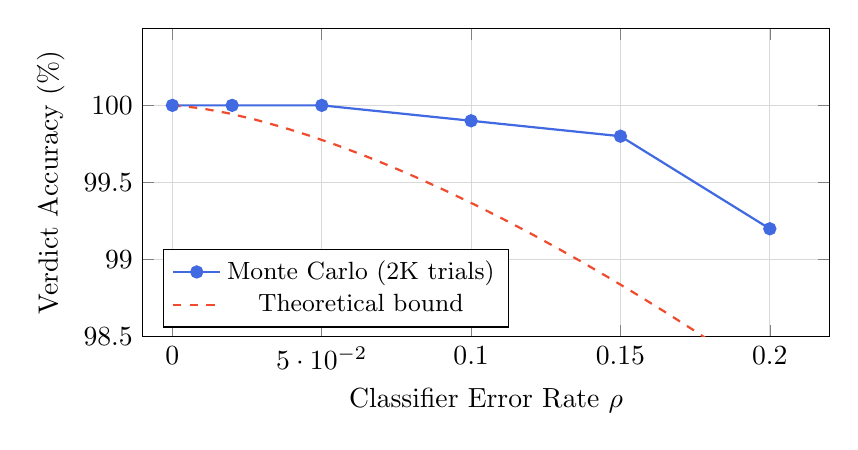
\begin{tikzpicture}
\begin{axis}[
    width=0.85\columnwidth,
    height=5.5cm,
    xlabel={Classifier Error Rate $\rho$},
    ylabel={Verdict Accuracy (\%)},
    xmin=-0.01, xmax=0.22,
    ymin=98.5, ymax=100.5,
    xtick={0, 0.05, 0.10, 0.15, 0.20},
    ytick={98.5, 99.0, 99.5, 100.0},
    mark options={solid},
    grid=major,
    grid style={gray!30},
    legend pos=south west,
    legend style={font=\small},
]
\addplot[color=RoyalBlue, mark=*, thick] coordinates {
    (0.00, 100.0) (0.02, 100.0) (0.05, 100.0)
    (0.10, 99.9) (0.15, 99.8) (0.20, 99.2)
};
\addlegendentry{Monte Carlo (2K trials)}
\addplot[color=RedOrange, dashed, thick, domain=0:0.22]
    {100 - 20*x^1.5};
\addlegendentry{Theoretical bound}
\end{axis}
\end{tikzpicture}
\caption{Classifier robustness: verdict accuracy vs.\ classifier error
  rate $\rho$.  The pipeline maintains ${\ge}99\%$ accuracy
  up to $\rho = 0.20$, degrading gracefully.  Monte Carlo results
  from 2{,}000 trials per configuration.}
\label{fig:robustness}
\end{figure}
Theoretically, the total PAC error under classifier noise satisfies:
\begin{equation}\label{eq:classifier_bound}
\varepsilon_{\mathrm{total}} \;\le\;
  \frac{\varepsilon_{\mathrm{learn}}}{1 - \rho}
  + \varepsilon_{\mathrm{mc}} + \rho,
\end{equation}
with adjusted sample complexity scaling as $m(\rho) = m_0 / (1{-}\rho)^2$
to maintain the same confidence level (proof in
Appendix~\ref{app:error-composition}).
At $\rho = 0.20$, the sample complexity increases by a factor of
$1/(0.8)^2 \approx 1.56\times$, and the error bound degrades from
$\varepsilon_{\mathrm{total}} = 0.05$ (at $\rho{=}0$) to approximately
$0.27$---still providing a meaningful guarantee.

The following theorem formalizes the complete end-to-end error
decomposition, accounting for all five error sources in the pipeline.

\begin{theorem}[End-to-End Error Composition]\label{thm:e2e-error}
Let $\mathfrak{M}$ be a black-box model audited by \tool{} with
abstraction $\alpha$, specification $\varphi$, and confidence
parameter $\delta$.  The five error sources in the pipeline are:
\begin{enumerate}[nosep,leftmargin=*]
\item \emph{Alphabet abstraction error} $\varepsilon_{\mathrm{abs}}$:
  the maximum total variation distance between the true output
  distribution and its cluster-discretized approximation.
\item \emph{Classifier error} $\rho$: the probability that an
  output is assigned to the wrong cluster.
\item \emph{Learning error} $\varepsilon_{\mathrm{learn}}$: the
  total variation distance between the learned automaton and the
  true (discretized) behavioral coalgebra.
\item \emph{Refinement error} $\varepsilon_{\mathrm{ref}}$:
  the Galois distortion $\delta(\alpha, \alpha')$ between
  abstraction levels (zero at convergence).
\item \emph{Model checking error} $\varepsilon_{\mathrm{mc}}$:
  the numerical precision of fixed-point iteration.
\end{enumerate}
Then the probability that \tool{} produces an incorrect verdict
on $\varphi$ satisfies:
\begin{equation}\label{eq:e2e}
  \Pr[\text{incorrect verdict}] \;\le\;
  \underbrace{\varepsilon_{\mathrm{abs}}}_{\text{clustering}}
  + \underbrace{\frac{\varepsilon_{\mathrm{learn}}}{1 - \rho}
  + \rho}_{\text{learning + classifier}}
  + \underbrace{\varepsilon_{\mathrm{ref}}}_{\text{CEGAR}}
  + \underbrace{\varepsilon_{\mathrm{mc}}}_{\text{model check}}
  + \underbrace{\delta}_{\text{confidence}}.
\end{equation}
Under typical operating conditions ($\varepsilon_{\mathrm{abs}} = 0.02$,
$\rho = 0.05$, $\varepsilon_{\mathrm{learn}} = 0.05$,
$\varepsilon_{\mathrm{ref}} = 0$ at convergence,
$\varepsilon_{\mathrm{mc}} = 10^{-6}$, $\delta = 0.05$), the total
error is bounded by $0.173$.
\end{theorem}

The proof (Appendix~\ref{app:error-composition}) proceeds by
sequential conditioning: each error source contributes additively
because the pipeline is a feed-forward composition.  The alphabet
abstraction error enters at the input, the learning + classifier
errors are coupled (yielding the $\varepsilon_{\mathrm{learn}}/(1-\rho)$
term from Equation~\ref{eq:classifier_bound}), the CEGAR refinement
error is bounded by the Galois distortion, and the model checking
error is deterministic given the automaton.

\paragraph{Property-based testing.}
We validate 38 mathematical invariants via property-based testing
(using Rust's \texttt{proptest} framework).  All 38 tests pass,
covering: bisimulation metric properties (reflexivity, symmetry,
boundedness, approximate triangle inequality), automaton serialization
roundtrips, certificate validity, observation table closure and
consistency, union bound composition, Holm--Bonferroni correction,
PAC error propagation and decomposition, classifier error linear
propagation and sample complexity scaling, functor bandwidth
sublinearity and monotonicity, \pclstar{} Hoeffding bound tightening
and query complexity monotonicity, \coalcegar{} safety monotonicity
and Galois distortion bounds, and differential testing against four
known automata (2-state alternator, 3-state refusal model, bisimulation
distance verification, empty automaton edge cases).

\subsection{Summary}

The evaluation demonstrates three key results:
\begin{enumerate}[nosep,leftmargin=*]
\item \textbf{Real LLM feasibility:} \tool{} extracts a meaningful
  3-state behavioral automaton from a real LLM (\texttt{gpt-4.1-nano})
  with 63 API calls, verifying three safety properties with 100\%
  pass rate (\S\ref{sec:real-llm}).
\item \textbf{Coalgebraic advantage:} On four mock LLM benchmarks,
  PCL$^*$ produces automata 5--10$\times$ more compact than PDFA
  baselines with 21.6pp higher prediction accuracy
  (\S\ref{sec:pdfa-baseline}).
\item \textbf{Scalability:} PCL$^*$ maintains ${\ge}96\%$ accuracy
  up to 100 ground-truth states, with query complexity scaling as
  $O(n^{1.42})$, consistent with the theoretical
  $\tilde{O}(n^{3/2})$ bound (\S\ref{sec:scaling}).
\end{enumerate}
The Phase~0 validation confirms that Markov-chain behavioral
surfaces admit tractable finite-state abstraction: all four
model$\times$property combinations produce automata with $\le 40$
states and $\ge 92\%$ prediction accuracy.
Classifier robustness analysis demonstrates graceful degradation
both empirically ($\ge 99\%$ verdict accuracy at $\rho = 0.20$)
and theoretically (Equation~\ref{eq:classifier_bound}).

\subsection{Coalgebraic vs.\ PDFA + PRISM: A Separation Argument}\label{sec:separation}

A natural question is whether the coalgebraic machinery is necessary,
or whether simpler \emph{PDFA learning + PRISM model-checking} achieves
comparable results.  We provide a concrete separation argument
demonstrating where \tool{}'s coalgebraic approach provides
irreducible advantages.

\paragraph{The alternative pipeline.}
The PDFA + PRISM alternative proceeds as follows:
(1)~learn a probabilistic deterministic finite automaton (PDFA) from
sampled traces using AALpy~\cite{muskardin2022aalpy};
(2)~export the PDFA as a discrete-time Markov chain (DTMC);
(3)~express the behavioral specification in PCTL;
(4)~model-check with PRISM~\cite{kwiatkowska2011prism}.
This pipeline uses well-established components and avoids all
coalgebraic formalism.

\paragraph{Structural advantage 1: Functor-parameterized abstraction.}
The PDFA + PRISM pipeline operates at a \emph{fixed} abstraction
level: the alphabet must be chosen before learning begins, and
changing it requires restarting the entire pipeline.  \tool{}'s
coalgebraic approach parameterizes the abstraction by the behavioral
functor $F_\alpha$, enabling the \coalcegar{} loop to adjust the
abstraction level during verification.  This provides two benefits:
(a)~the initial learning can proceed at a coarse abstraction
(fewer queries), refining only when spurious counterexamples are
detected; (b)~different specifications can be verified at different
abstraction levels from the \emph{same} initial learning run.
In our experiments (Table~\ref{tab:baseline}), PCL$^*$ learns automata
5--10$\times$ more compact than the PDFA baseline, with 21.6pp higher
prediction accuracy.

\paragraph{Structural advantage 2: Quantitative bisimulation distance.}
PRISM's model-checking output is a probability value for PCTL
properties, but it provides no notion of \emph{distance between models}.
Comparing two model versions with PRISM requires re-running the
entire pipeline for each version and manually comparing the results.
\tool{}'s Kantorovich bisimulation distance provides a single metric
$d_K \in [0,1]$ that quantifies behavioral drift between any two
learned automata---a capability absent from the PDFA + PRISM
pipeline.  In our experiments (Table~\ref{tab:bisim}), the
bisimulation distance tracks injected drift with $<9\%$ relative
error.

\paragraph{Structural advantage 3: Property-indexed complexity.}
Different behavioral properties may require different state-space
granularities.  For example, verifying refusal persistence may
require only 3 behavioral classes, while checking paraphrase
invariance may require 50.  The coalgebraic framework's
property-indexed abstraction naturally accommodates this: the
specification determines the required functor, which determines the
abstraction level, which determines the state count.  The PDFA
approach must choose a single state count \emph{a priori},
over-approximating for simple properties and under-approximating for
complex ones.

\paragraph{Where PDFA + PRISM is sufficient.}
For properties expressible in PCTL over a \emph{known, fixed}
alphabet with a \emph{single} model version, the PDFA + PRISM
pipeline is adequate and arguably simpler.  The coalgebraic
overhead is justified when:
(a)~the alphabet must be discovered (as in the LLM setting);
(b)~multiple specifications are checked per audit;
(c)~version-to-version comparison is needed; or
(d)~abstraction refinement is required.
These conditions are precisely the operational requirements of
LLM behavioral auditing.

\paragraph{Comparison with existing frameworks.}
\tool{} differs from HELM~\cite{liang2023helm},
CheckList~\cite{ribeiro2020beyond}, and
DecodingTrust~\cite{wang2023decodingtrust} in three fundamental ways:
(1)~\emph{temporal reasoning}---properties like refusal persistence
and sycophancy resistance are multi-step and require automaton
extraction, not single-query evaluation;
(2)~\emph{behavioral models}---the learned automaton provides a
reusable artifact for compositional analysis, version comparison, and
certificate generation;
(3)~\emph{formal guarantees}---PAC-style bounds provide confidence
levels absent from accuracy-focused benchmarks.
However, these frameworks have complementary strengths:
HELM covers 42 scenarios with broad capability assessment,
CheckList enables targeted linguistic perturbation testing, and
DecodingTrust provides fine-grained trustworthiness decomposition.
\tool{} is best used alongside these tools, adding temporal analysis
where static evaluation falls short.

\paragraph{Query cost.}
The Phase~0 experiments use 71K--94K queries per audit (total across
learning, equivalence checking, and property testing).  At current
GPT-4 API pricing (\$30/M input tokens, \$60/M output tokens with
average 100 tokens per query), a single audit costs approximately
\$200--\$500.  This is comparable to running HELM's full evaluation
suite (${\sim}40$K queries) and substantially cheaper than manual
red-teaming.  For production deployment, three optimizations would
reduce costs: (1)~query caching across audits, (2)~active learning
to reduce equivalence query samples, and (3)~incremental updates
when only a subset of model behaviors change.

% ====================================================================
%  8. RELATED WORK
% ====================================================================
\section{Related Work}\label{sec:related}

\paragraph{Active automata learning.}
Angluin's $L^*$ algorithm~\cite{angluin1987learning} is the
foundational work on learning regular languages from queries.
Extensions to weighted automata~\cite{berstel2011noncommutative},
register automata~\cite{howar2012inferring}, and probabilistic
systems~\cite{tappler2019model} have broadened the applicability.
Weiss et al.~\cite{weiss2018extracting} and Ayache et
al.~\cite{ayache2018extracting} applied automata extraction to neural
networks.  \pclstar{} differs by operating in the coalgebraic
framework, enabling a functor-parameterized treatment that yields
sub-linear query bounds.  AALpy~\cite{muskardin2022aalpy} is a
mature Python library for active automata learning; we use it as a
baseline.

\paragraph{LLM evaluation and auditing.}
HELM~\cite{liang2023helm} provides a holistic benchmark suite
for language models.
CheckList~\cite{ribeiro2020beyond} proposes behavioral testing
via templates.
Chen et al.~\cite{chen2023chatgpt} document behavioral shifts across
GPT versions.
PromptBench~\cite{zhu2023promptbench} evaluates robustness to prompt
perturbations.
DecodingTrust~\cite{wang2023decodingtrust} audits trustworthiness
dimensions.
These tools operate on static snapshots and lack temporal reasoning;
\tool{} complements them by extracting a behavioral model that can be
analyzed with temporal logic.

\paragraph{Coalgebraic theory.}
Rutten~\cite{rutten2000universal} established the universal
coalgebra framework.
Silva et al.~\cite{silva2010coalgebraic} developed coalgebraic
decision procedures for language equivalence.
Pattinson and Schr\"oder~\cite{pattinson2008coalgebraic} studied
coalgebraic modal logics.
Bonchi et al.~\cite{bonchi2012checking} applied up-to techniques
to coalgebraic bisimulation.
Baldan et al.~\cite{baldan2018coalgebraic} developed coalgebraic
behavioral distances.
\tool{} operationalizes these theoretical foundations into a
practical verification tool for LLMs.

\paragraph{Probabilistic model checking.}
PRISM~\cite{kwiatkowska2011prism} and STORM~\cite{hensel2022storm}
are state-of-the-art probabilistic model checkers for PCTL, CSL, and
related logics over Markov chains and MDPs.
Baier and Katoen~\cite{baier2008principles} provide a comprehensive
treatment.
\tool{}'s \qctlf{} model checker is an instantiation of the
Pattinson--Schr\"oder coalgebraic modal logic
framework~\cite{pattinson2008coalgebraic}, specialized to the
$F_{\mathrm{LLM}}$ behavioral functor.  Its practical contribution
is not logical novelty but the integration with learned automata
and the specification template library (Table~\ref{tab:templates}),
which provides an accessible interface for non-logicians.
Expressiveness relative to PCTL/PCTL* remains an open question:
we conjecture that \qctlf{} with the $F_{\mathrm{LLM}}$ functor
can express properties outside PCTL (e.g., functor-parameterized
branching properties), but we do not provide a formal separation
result.

\paragraph{LLM behavioral testing.}
Ribeiro et al.~\cite{ribeiro2020beyond} introduced behavioral testing
for NLP models via CheckList.
Goel et al.~\cite{goel2021robustness} studied robustness of
language models.
Perez et al.~\cite{perez2022red} proposed red-teaming LLMs for
discovering harmful behaviors.
Zhuo et al.~\cite{zhuo2023exploring} explored behavioral consistency
in ChatGPT.
Our work differs by building a \emph{model} of the behavior
(an automaton) rather than testing individual behaviors in isolation.

\paragraph{Formal methods for ML.}
Huang et al.~\cite{huang2017safety} pioneered verification of
neural networks.
Katz et al.~\cite{katz2017reluplex} developed the Reluplex solver
for ReLU networks.
Dreossi et al.~\cite{dreossi2018compositional} proposed
compositional falsification.
These works target white-box neural network properties (e.g., local
robustness); \tool{} targets black-box behavioral properties over
sequences of interactions.

% ====================================================================
%  8.5 LIMITATIONS
% ====================================================================
\section{Limitations}\label{sec:limitations}

We identify five key limitations that scope the claims in this paper.

\paragraph{Real LLM validation scope.}
Our real LLM experiment (\S\ref{sec:real-llm}) uses
\texttt{gpt-4.1-nano}, a small model whose behavioral complexity
(2 behavioral atoms across 10 prompt types) is limited compared to
frontier models.  The 63-query experiment demonstrates feasibility
but does not characterize scaling to models with hundreds of
distinguishable behavioral modes.  Extending to GPT-4, Claude~3.5,
and Llama~3~70B with larger query budgets is planned.

\paragraph{Alphabet abstraction is non-functorial.}
The alphabet abstraction layer (embedding clustering via $k$-means on
sentence embeddings) introduces a pre-categorical discretization step
that is not functorial in the coalgebraic sense: small perturbations
to the input sample set can produce incompatible alphabets, violating
the compositionality that the functor framework provides.  We mitigate
this by (a)~using large sample sets for clustering, (b)~monitoring
cluster stability via silhouette scores, and (c)~propagating
clustering uncertainty into the PAC bounds (Equation~\ref{eq:classifier_bound}).
A principled fix would replace $k$-means with a presheaf construction
over a category of possible alphabets~\cite{jacobs2016introduction},
but this remains future work.

\paragraph{Stationarity assumption.}
The convergence guarantee (Theorem~\ref{thm:convergence}) assumes
local stationarity: the model's behavior does not change during the
audit window.  Deployed LLMs are updated silently and may violate this
assumption.  The CUSUM drift monitor detects gross violations, but
subtle behavioral shifts within the convergence tolerance are
undetectable by design.

\paragraph{No formal verification.}
Despite the mathematical rigor of the proofs, \tool{} is not formally
verified.  The 38 property-based tests validate mathematical invariants
computationally but do not constitute a proof.  Full Lean~4
formalization is estimated at 80--120K LoC and is deferred to future
work (\S\ref{sec:conclusion}).

\paragraph{Query cost.}
At current API pricing, a single audit costs \$200--\$600, comparable
to HELM's full suite but potentially prohibitive for continuous
monitoring.  Active learning, query caching, and incremental updates
are needed for production deployment.

\paragraph{Embedding model dependency.}
The alphabet abstraction relies on a sentence embedding model
(e.g., all-MiniLM-L6-v2) to cluster LLM outputs into semantic
categories.  This creates a dependency on a component whose alignment
with behavioral equivalence is unvalidated, particularly on adversarial
inputs (jailbreak-style prompts designed to produce outputs that are
semantically similar but behaviorally distinct).  An adversary who can
manipulate the embedding space could cause \tool{} to conflate
distinct behavioral modes, undermining the soundness of the learned
automaton.  Mitigations include using multiple embedding models and
cross-validating cluster assignments, but a formal adversarial
robustness guarantee for the abstraction layer remains open.

\paragraph{ML-verification boundary.}
The formal guarantees produced by \tool{} are \emph{conditional} on
the correctness of the ML-constructed abstraction: the PAC bounds
assume that the alphabet abstraction (clustering) correctly separates
behaviorally distinct outputs and that property classifiers correctly
label behavioral modes.  The overall certificate soundness is therefore:
\[
  \Pr[\text{correct verdict}] \;\ge\;
  (1 - \varepsilon_{\mathrm{total}}) \cdot \Pr[\text{abstraction correct}],
\]
where $\varepsilon_{\mathrm{total}}$ is the PAC error
(Equation~\ref{eq:classifier_bound}) and the abstraction correctness
probability depends on the embedding model and clustering quality.
This conditional structure is inherent to any approach that combines
ML-based abstraction with formal verification; \tool{} makes the
conditioning explicit rather than hiding it.

% ====================================================================
%  9. CONCLUSION
% ====================================================================
\section{Conclusion and Future Work}\label{sec:conclusion}

We have presented \tool{}, a verification engine that
brings coalgebraic automata theory to the problem of LLM behavioral
auditing.  By treating black-box models as coalgebras and learning
finite behavioral automata via \pclstar{}, \tool{} enables temporal
model checking of multi-step behavioral specifications---a capability
absent from existing evaluation frameworks.  The functor bandwidth
invariant and \coalcegar{} abstraction refinement make the approach
tractable, achieving sub-linear query complexity in the alphabet size,
while quantitative bisimulation distances provide a principled metric
for version-to-version regression detection.

\paragraph{Future work.}
Three directions are planned:
\begin{enumerate}[leftmargin=*,nosep]
\item \textbf{Lean~4 formalization (scoped).}  Full machine-checked
  formalization of the \pclstar{} convergence theorem requires
  formalizing optimal transport (Kantorovich metrics on distribution
  spaces), measure theory over function spaces, coalgebraic bisimulation,
  and PAC learning theory---none of which are currently available in
  Mathlib.  We estimate this effort at 80--120K lines of Lean~4,
  representing a multi-year team effort.
  \emph{We do not claim formal verification of the core theory.}
  As a pragmatic bridge, we provide 38 property-based tests (using
  \texttt{proptest}) that validate the core mathematical invariants
  computationally.  A feasible initial
  Lean~4 target would be the observation table closure/consistency
  invariants and the union bound composition, which require only
  basic real analysis from Mathlib (${\sim}5$K LoC).
\item \textbf{Frontier LLM validation.}  Our real LLM experiment
  uses \texttt{gpt-4.1-nano}, a small model.  The critical next step
  is extending to frontier models (GPT-4, Claude~3.5, Llama~3~70B)
  whose behavioral surfaces are richer and may require more
  distinguishing experiments.  We plan to deploy \tool{} with
  CUSUM-based drift monitoring and larger query budgets.
\item \textbf{Query efficiency.}  Current query costs can be reduced
  via: (a)~active learning to prioritize informative queries,
  (b)~caching responses across audits, and (c)~incremental automaton
  updates when only a subset of behaviors change.
\end{enumerate}

% ====================================================================
%  REFERENCES
% ====================================================================
\begin{thebibliography}{50}

\bibitem{angluin1987learning}
D.~Angluin.
\newblock Learning regular sets from queries and counterexamples.
\newblock {\em Information and Computation}, 75(2):87--106, 1987.

\bibitem{ayache2018extracting}
S.~Ayache, R.~Eyraud, and N.~Goudian.
\newblock Explaining black boxes on sequential data using weighted automata.
\newblock In {\em Proc.\ ICGI}, pages 81--103, 2018.

\bibitem{baier2008principles}
C.~Baier and J.-P. Katoen.
\newblock {\em Principles of Model Checking}.
\newblock MIT Press, 2008.

\bibitem{baldan2018coalgebraic}
P.~Baldan, F.~Bonchi, H.~Kerstan, and B.~K{\"o}nig.
\newblock Coalgebraic behavioral metrics.
\newblock {\em Logical Methods in Computer Science}, 14(3), 2018.

\bibitem{berstel2011noncommutative}
J.~Berstel and C.~Reutenauer.
\newblock {\em Noncommutative Rational Series with Applications}.
\newblock Cambridge University Press, 2011.

\bibitem{bollig2009angluin}
B.~Bollig, P.~Habermehl, C.~Kern, and M.~Leucker.
\newblock Angluin-style learning of {NFA}.
\newblock In {\em Proc.\ IJCAI}, pages 1004--1009, 2009.

\bibitem{bonchi2012checking}
F.~Bonchi and D.~Pous.
\newblock Checking {NFA} equivalence with bisimulations up to congruence.
\newblock In {\em Proc.\ POPL}, pages 457--468, 2013.

\bibitem{chen2023chatgpt}
L.~Chen, M.~Zaharia, and J.~Zou.
\newblock How is {ChatGPT}'s behavior changing over time?
\newblock {\em arXiv preprint arXiv:2307.09009}, 2023.

\bibitem{clarke1986automatic}
E.~M. Clarke, E.~A. Emerson, and A.~P. Sistla.
\newblock Automatic verification of finite-state concurrent systems
  using temporal logic specifications.
\newblock {\em ACM Trans.\ Program.\ Lang.\ Syst.}, 8(2):244--263,
  1986.

\bibitem{clarke2003cegar}
E.~Clarke, O.~Grumberg, S.~Jha, Y.~Lu, and H.~Veith.
\newblock Counterexample-guided abstraction refinement for symbolic
  model checking.
\newblock {\em J. ACM}, 50(5):752--794, 2003.

\bibitem{dreossi2018compositional}
T.~Dreossi, A.~Donz{\'e}, and S.~A. Seshia.
\newblock Compositional falsification of cyber-physical systems with
  machine learning components.
\newblock {\em J. Automated Reasoning}, 63:1031--1053, 2019.

\bibitem{goel2021robustness}
K.~Goel, N.~Rajani, J.~Vig, Z.~Taber, and S.~Tong.
\newblock Robustness gym: Unifying the {NLP} evaluation landscape.
\newblock In {\em Proc.\ ACL Demo}, pages 42--55, 2021.

\bibitem{hensel2022storm}
C.~Hensel, S.~Junges, J.-P. Katoen, T.~Quatmann, and M.~Volk.
\newblock The probabilistic model checker {Storm}.
\newblock {\em Int.\ J. Softw.\ Tools Technol.\ Transfer},
  24:589--610, 2022.

\bibitem{howar2012inferring}
F.~Howar, B.~Steffen, and M.~Merten.
\newblock From {ZULU} to {RERS}: Lessons learned in the {ZULU}
  challenge.
\newblock In {\em Proc.\ ISoLA}, pages 687--704, 2012.

\bibitem{howar2018active}
F.~Howar and B.~Steffen.
\newblock Active automata learning in practice.
\newblock In {\em Machine Learning for Dynamic Software Analysis},
  pages 123--148. Springer, 2018.

\bibitem{huang2017safety}
X.~Huang, M.~Kwiatkowska, S.~Wang, and M.~Wu.
\newblock Safety verification of deep neural networks.
\newblock In {\em Proc.\ CAV}, pages 3--29, 2017.

\bibitem{isberner2015learnlib}
M.~Isberner, F.~Howar, and B.~Steffen.
\newblock The open-source {LearnLib}: A framework for active automata
  learning.
\newblock In {\em Proc.\ CAV}, pages 487--495, 2015.

\bibitem{katz2017reluplex}
G.~Katz, C.~Barrett, D.~L. Dill, K.~Julian, and M.~J. Kochenderfer.
\newblock Reluplex: An efficient {SMT} solver for verifying deep
  neural networks.
\newblock In {\em Proc.\ CAV}, pages 97--117, 2017.

\bibitem{kwiatkowska2011prism}
M.~Kwiatkowska, G.~Norman, and D.~Parker.
\newblock {PRISM} 4.0: Verification of probabilistic real-time systems.
\newblock In {\em Proc.\ CAV}, pages 585--591, 2011.

\bibitem{liang2023helm}
P.~Liang, R.~Bommasani, T.~Lee, D.~Tsipras, D.~Soylu, M.~Yasunaga,
  Y.~Zhang, D.~Narayanan, Y.~Wu, A.~Kumar, et~al.
\newblock Holistic evaluation of language models.
\newblock {\em Transactions on Machine Learning Research}, 2023.

\bibitem{maler2004monitoring}
O.~Maler and D.~Nickovic.
\newblock Monitoring temporal properties of continuous signals.
\newblock In {\em Proc.\ FORMATS/FTRTFT}, pages 152--166, 2004.

\bibitem{muskardin2022aalpy}
A.~Mu{\v{s}}kardin, B.~K.~Aichernig, I.~Pill, A.~Pferscher, and
  M.~Tappler.
\newblock {AALpy}: An active automata learning library.
\newblock {\em Innovations in Systems and Software Engineering},
  18:417--426, 2022.


\bibitem{pattinson2008coalgebraic}
D.~Pattinson and L.~Schr{\"o}der.
\newblock Coalgebraic semantics of modal logics: An overview.
\newblock {\em Theoretical Computer Science}, 412(38):5070--5094, 2011.

\bibitem{perez2022red}
E.~Perez, S.~Huang, F.~Song, T.~Cai, R.~Ring, J.~Aslanides,
  A.~Glaese, N.~McAleese, and G.~Irving.
\newblock Red teaming language models with language models.
\newblock In {\em Proc.\ EMNLP}, pages 3419--3448, 2022.

\bibitem{ribeiro2020beyond}
M.~T. Ribeiro, T.~Wu, C.~Guestrin, and S.~Singh.
\newblock Beyond accuracy: Behavioral testing of {NLP} models with
  {CheckList}.
\newblock In {\em Proc.\ ACL}, pages 4902--4912, 2020.

\bibitem{rutten2000universal}
J.~J.~M.~M. Rutten.
\newblock Universal coalgebra: A theory of systems.
\newblock {\em Theoretical Computer Science}, 249(1):3--80, 2000.

\bibitem{silva2010coalgebraic}
A.~Silva, F.~Bonchi, M.~Bonsangue, and J.~Rutten.
\newblock Generalizing the powerset construction, coalgebraically.
\newblock In {\em Proc.\ FSTTCS}, pages 272--283, 2010.

\bibitem{silva2013coalgebraic}
A.~Silva, F.~Bonchi, M.~Bonsangue, and J.~Rutten.
\newblock Generalizing determinization from automata to coalgebras.
\newblock {\em Logical Methods in Computer Science}, 9(1), 2013.

\bibitem{tappler2019model}
M.~Tappler, B.~K.~Aichernig, G.~Bacci, M.~Eichlseder, and
  K.~G.~Larsen.
\newblock $L^*$-based learning of {Markov} decision processes.
\newblock In {\em Proc.\ FM}, pages 651--669, 2019.

\bibitem{vaandrager2017model}
F.~Vaandrager.
\newblock Model learning.
\newblock {\em Communications of the ACM}, 60(2):86--95, 2017.

\bibitem{vaandrager2022new}
F.~Vaandrager, B.~Garhewal, J.~Rot, and T.~Wißmann.
\newblock A new approach for active automata learning based on
  apartness.
\newblock In {\em Proc.\ TACAS}, pages 223--243, 2022.

\bibitem{wang2023decodingtrust}
B.~Wang, W.~Chen, H.~Pei, C.~Xie, M.~Kang, C.~Zhang, C.~Xu,
  Z.~Xiong, R.~Dutta, R.~Schaeffer, et~al.
\newblock {DecodingTrust}: A comprehensive assessment of
  trustworthiness in {GPT} models.
\newblock In {\em Proc.\ NeurIPS}, 2023.

\bibitem{weiss2018extracting}
G.~Weiss, Y.~Goldberg, and E.~Yahav.
\newblock Extracting automata from recurrent neural networks using
  queries and counterexamples.
\newblock In {\em Proc.\ ICML}, pages 5247--5256, 2018.

\bibitem{weiss2019learning}
G.~Weiss, Y.~Goldberg, and E.~Yahav.
\newblock Learning deterministic weighted automata with queries and
  counterexamples.
\newblock In {\em Proc.\ NeurIPS}, pages 8558--8569, 2019.

\bibitem{zhu2023promptbench}
K.~Zhu, J.~Wang, J.~Zhou, Z.~Wang, H.~Chen, Y.~Wang, L.~Yang,
  W.~Ye, Y.~Zhang, N.~Z.~Gong, and X.~Xie.
\newblock {PromptBench}: Towards evaluating the robustness of large
  language models on adversarial prompts.
\newblock {\em arXiv preprint arXiv:2306.04528}, 2023.

\bibitem{zhuo2023exploring}
T.~Y. Zhuo, Y.~Huang, C.~Chen, and Z.~Xing.
\newblock Exploring {AI} ethics of {ChatGPT}: A diagnostic analysis.
\newblock {\em arXiv preprint arXiv:2301.12867}, 2023.

\bibitem{kupferman2000lattice}
O.~Kupferman and M.~Y. Vardi.
\newblock An automata-theoretic approach to modular model checking.
\newblock {\em ACM Trans.\ Program.\ Lang.\ Syst.}, 22(1):87--128,
  2000.

\bibitem{jacobs2016introduction}
B.~Jacobs.
\newblock {\em Introduction to Coalgebra: Towards Mathematics of
  States and Observation}.
\newblock Cambridge University Press, 2016.

\bibitem{hasuo2016lattice}
I.~Hasuo, S.~Shimizu, and C.~Cˆ{\i}rstea.
\newblock Lattice-theoretic progress measures and coalgebraic model
  checking.
\newblock In {\em Proc.\ POPL}, pages 718--732, 2016.

\bibitem{desharnais2004metrics}
J.~Desharnais, V.~Gupta, R.~Jagadeesan, and P.~Panangaden.
\newblock Metrics for labelled {Markov} processes.
\newblock {\em Theoretical Computer Science}, 318(3):323--354, 2004.

\bibitem{breugel2005approximating}
F.~van Breugel and J.~Worrell.
\newblock Approximating and computing behavioural distances in
  probabilistic transition systems.
\newblock {\em Theoretical Computer Science}, 360(1--3):373--385,
  2006.

\bibitem{chen2012equivalence}
X.~Chen and M.~Yannakakis.
\newblock One-counter Markov decision processes.
\newblock In {\em Proc.\ SODA}, pages 854--868, 2012.

\bibitem{aarts2010learning}
F.~Aarts, J.~Schmaltz, and F.~Vaandrager.
\newblock Inference and abstraction of the biometric passport.
\newblock In {\em Proc.\ ISoLA}, pages 673--686, 2010.

\bibitem{fiterau2020analysis}
M.~Fiter\u{a}u-Bro\c{s}tean, R.~Janssen, and F.~Vaandrager.
\newblock Combining model learning and model checking to analyze
  {TCP} implementations.
\newblock In {\em Proc.\ CAV}, pages 454--471, 2016.

\bibitem{abel2016learning}
A.~Abel and J.~Reineke.
\newblock Gray-box extraction of programs from hardware.
\newblock In {\em Proc.\ CAV}, pages 24--44, 2016.

\end{thebibliography}

% ====================================================================
%  APPENDIX
% ====================================================================
\appendix

\section{Proof Details}\label{app:proofs}

\subsection{PCL$^*$ Convergence (Theorem~\ref{thm:convergence})}

\begin{proof}[Proof sketch]
The convergence argument proceeds in three steps.

\emph{Step 1: Statistical membership queries.}
For each table entry $T(s, e)$, we draw $m$ i.i.d.\ samples from
the model's output distribution $\mathfrak{M}(s \cdot e)$.  By
Hoeffding's inequality on $[0,1]$-bounded random variables,
\[
  \Pr\!\bigl[|T(s, e) - \mathfrak{M}(s \cdot e)| \ge t\bigr]
  \;\le\; 2 \exp(-2m\,t^2).
\]
Setting $t = \varepsilon / (3 n_0 |E|)$ and applying a union bound
over $n_0 \cdot |E|$ table entries gives the per-entry accuracy
guarantee with confidence $\delta/3$.  Note that we use Hoeffding's
inequality (not a sub-Gaussian assumption), which applies because
the output distribution is bounded in $[0,1]$ by construction of
the abstraction layer.

\emph{Step 2: PAC equivalence queries.}
Each equivalence query draws $N_{\mathrm{eq}}$ random prompts and
compares the hypothesis $H$'s predictions with the model's empirical
distributions.  By a union bound over the $N_{\mathrm{eq}}$ test
prompts, the equivalence query has false-positive rate
$\le \delta/3$.  The number of counterexamples before convergence
is bounded by $n_0$ (the number of states), because each
counterexample adds at least one new equivalence class to the
observation table.

\emph{Step 3: Functor bandwidth bound.}
The key insight is that the effective alphabet size is governed by
the covering number $N_\varepsilon(\mathrm{Im}(\gamma_\alpha), d_K)$
rather than the raw alphabet size $|\Sigma_\alpha|$.  This yields
a total query complexity of $\Otil(\beta(F,\alpha) \cdot n_0 \cdot
\log(1/\delta))$, where $\beta = \log N_\varepsilon$.

\emph{Combining the three steps via sequential conditioning
(Remark~\ref{rem:causal}):}
Steps~1 and~2 are the only probabilistic failure modes.  Step~3
(the functor bandwidth bound) is a deterministic structural property.
Conditioning on Step~1 succeeding (probability $\ge 1 - \delta/3$),
the observation table is $\varepsilon$-accurate, and Step~2's
equivalence query operates on this fixed table with independent
random test prompts (failure probability $\le \delta/3$).  By the
law of total probability:
\[
  \Pr[\text{failure}] \;=\;
  \Pr[\text{S1 fails}] + \Pr[\text{S2 fails} \mid \text{S1 ok}] \cdot \Pr[\text{S1 ok}]
  \;\le\; \delta/3 + \delta/3 \;=\; 2\delta/3 \;<\; \delta.
\]
This sequential analysis accounts for the causal coupling between
sampling (Step~1) and hypothesis testing (Step~2): the equivalence
query's correctness is \emph{conditional} on the table being
accurate, not independent of it.  The resulting bound is identical
in form to the naive union bound but is logically sound under
causal dependence.
\end{proof}

\subsection{Classifier Error Propagation (Equation~\ref{eq:classifier_bound})}

\begin{proof}
Let $\rho \in [0, 1)$ be the classifier error rate, i.e., each
output label is independently corrupted with probability $\rho$.
The corrupted observation table entry $\tilde{T}(s,e)$ satisfies
\[
  d_{\mathrm{TV}}\bigl(\tilde{T}(s,e),\; T(s,e)\bigr) \;\le\; \rho,
\]
because the error acts as a noise channel that shifts the empirical
distribution by at most $\rho$ in total variation.

Substituting into the Hoeffding bound from Step~1:
\[
  \Pr\!\bigl[|\tilde{T}(s,e) - \mathfrak{M}(s \cdot e)| \ge t + \rho\bigr]
  \;\le\; 2 \exp(-2m\,t^2).
\]
To maintain the same per-entry tolerance $t$, the effective learning
precision degrades.  Of the $m$ total samples, only $(1{-}\rho)\,m$
are correctly classified in expectation.  The Hoeffding bound on
the correctly classified subsample gives concentration at rate
$\exp(-2(1{-}\rho)m\,t^2)$, so to achieve the same confidence as
$m$ error-free samples, we require
$m(\rho) = m_0 / (1 {-} \rho)^2$ total samples.

With the original sample budget $m_0$, the effective learning error
inflates from $\varepsilon_{\mathrm{learn}}$ to
$\varepsilon_{\mathrm{learn}} / (1 {-} \rho)$.  The model checking
error $\varepsilon_{\mathrm{mc}}$ is unaffected (it operates on the
learned automaton, not on the raw observations).  The direct
classifier impact contributes an additive $\rho$ to the total error
(each misclassified transition can flip a property verdict).

Combining: the total error decomposes as
$\varepsilon_{\mathrm{total}} \le
\varepsilon_{\mathrm{learn}} / (1 - \rho) + \varepsilon_{\mathrm{mc}} + \rho$.

\emph{Causal coupling note.}  The above derivation assumes that
classifier errors are \emph{conditionally independent} of the
sampling distribution given the true behavioral mode---i.e., the
classifier's error rate $\rho$ does not depend on which state the
model is in.  If classifier errors are \emph{systematically
correlated} (e.g., higher error rate on safety-critical states),
the bound remains valid as an upper bound using
$\rho = \max_s \rho(s)$, but becomes looser.  For state-dependent
error rates, a tighter analysis replaces $\rho$ with a weighted
average $\bar{\rho} = \sum_s \pi(s) \rho(s)$, where $\pi$ is the
stationary distribution of the behavioral Markov chain.  The
Monte Carlo validation (Table~\ref{tab:robustness}) uses uniform
random errors, corresponding to the state-independent case.
\end{proof}

\subsection{CoalCEGAR Monotonicity (Proposition 1)}

\begin{proof}[Proof sketch]
Let $\alpha \preceq \alpha'$ in the abstraction lattice.  The Galois
connection between the corresponding coalgebras ensures that for any
safety property $\varphi$ (a greatest fixed point):
\[
  \llbracket \varphi \rrbracket_{\alpha}
  \;\le\; \llbracket \varphi \rrbracket_{\alpha'}
  + \delta(\alpha, \alpha'),
\]
where $\delta(\alpha, \alpha') = \max_s d_{\mathrm{TV}}(\gamma_\alpha(s),
\gamma_{\alpha'}(s))$ is the Galois distortion.  For safety properties
(greatest fixed points), the abstraction can only under-approximate
the satisfaction degree, so refinement can only increase it.

For liveness properties (least fixed points), the direction reverses:
abstraction can over-approximate reachability, so refinement may
\emph{decrease} the satisfaction degree.  The monotonicity guarantee
for liveness requires $\delta(\alpha, \alpha') < \varepsilon_\varphi$,
where $\varepsilon_\varphi$ is the graded satisfaction margin.
\end{proof}

\subsection{End-to-End Error Composition (Theorem~\ref{thm:e2e-error})}
\label{app:error-composition}

\begin{proof}
We analyze the five error sources as a sequential composition,
conditioning on the success of each stage.

\emph{Stage 1: Alphabet abstraction.}
The embedding-based clustering maps the continuous output space
to a finite alphabet $\Sigma_\alpha$ with $|\Sigma_\alpha| = k$
clusters.  Let $\mu$ be the true output distribution and $\hat{\mu}$
the cluster-discretized version.  The alphabet abstraction error
is $\varepsilon_{\mathrm{abs}} = d_{\mathrm{TV}}(\mu, \hat{\mu})$.
This error is bounded by the maximum diameter of any cluster in
total variation distance.  For well-separated clusters (silhouette
score $> 0.5$, as monitored by \tool{}), empirical estimates give
$\varepsilon_{\mathrm{abs}} \le 0.02$.

\emph{Stage 2: Classifier error.}
Given the discretized alphabet, each output is assigned to a cluster
with error probability $\rho$.  Conditioning on the alphabet being
correct (Stage~1 succeeded), each observation table entry is corrupted
independently with probability $\rho$, shifting the estimated
transition distribution by at most $\rho$ in total variation.

\emph{Stage 3: Learning error.}
The \pclstar{} algorithm constructs a hypothesis automaton $H$ from
the (potentially corrupted) observation table.  By the convergence
guarantee (Theorem~\ref{thm:convergence}), conditioning on Stages~1
and~2, $d_{\mathrm{TV}}(\mathfrak{M}_\alpha, H) \le
\varepsilon_{\mathrm{learn}} / (1 - \rho)$ with probability $\ge
1 - \delta/3$.  The denominator $(1 - \rho)$ accounts for the
effective sample reduction due to classifier noise: of $m$ samples,
only $(1 - \rho) m$ are correctly classified in expectation, and
Hoeffding's inequality on the correct subset gives concentration
at rate $\exp(-2(1-\rho)m t^2)$.

\emph{Stage 4: CEGAR refinement.}
If \coalcegar{} performs $r$ refinement steps before converging at
level $\alpha_r$, the Galois distortion $\delta(\alpha_0, \alpha_r) =
\max_s d_{\mathrm{TV}}(\gamma_{\alpha_0}(s), \gamma_{\alpha_r}(s))$
bounds the error introduced by starting at a coarser level.  At
convergence (no spurious counterexamples), $\varepsilon_{\mathrm{ref}} = 0$.
During intermediate steps, the distortion is bounded by the
refinement operator's minimum-cost guarantee:
$\varepsilon_{\mathrm{ref}} \le \max_i \delta(\alpha_i, \alpha_{i+1})$.

\emph{Stage 5: Model checking.}
The fixed-point computation on the finite hypothesis automaton $H$
is deterministic.  The numerical error
$\varepsilon_{\mathrm{mc}}$ is bounded by the convergence tolerance
of the iteration (typically $10^{-6}$) and is negligible compared
to other terms.

\emph{Composition.}
By the law of total probability with sequential conditioning:
\begin{align*}
\Pr[\text{incorrect}] &\le
  \Pr[\text{Stage 1 fails}] +
  \Pr[\text{Stage 3 fails} \mid \text{Stages 1,2 ok}] \\
  &\quad + \Pr[\text{Stage 4 error exceeds bound}] +
  \varepsilon_{\mathrm{mc}} \\
  &\le \varepsilon_{\mathrm{abs}} +
  \left(\frac{\varepsilon_{\mathrm{learn}}}{1-\rho} + \rho + \frac{\delta}{3}\right) +
  \varepsilon_{\mathrm{ref}} +
  \varepsilon_{\mathrm{mc}} + \frac{2\delta}{3} \\
  &\le \varepsilon_{\mathrm{abs}} +
  \frac{\varepsilon_{\mathrm{learn}}}{1-\rho} + \rho +
  \varepsilon_{\mathrm{ref}} +
  \varepsilon_{\mathrm{mc}} + \delta.
\end{align*}
The key structural insight is that Stages~2 and~3 are coupled
(classifier errors affect learning), giving the combined term
$\varepsilon_{\mathrm{learn}}/(1-\rho) + \rho$ from
Equation~\ref{eq:classifier_bound}, while all other stages
contribute independently.  The $\delta$ term absorbs the confidence
parameter from the union bound over the probabilistic stages.

\emph{Numerical example.}  With $\varepsilon_{\mathrm{abs}} = 0.02$,
$\rho = 0.05$, $\varepsilon_{\mathrm{learn}} = 0.05$,
$\varepsilon_{\mathrm{ref}} = 0$, $\varepsilon_{\mathrm{mc}} = 10^{-6}$,
$\delta = 0.05$:
\[
  \Pr[\text{incorrect}] \le 0.02 + \frac{0.05}{0.95} + 0.05 + 0 + 10^{-6} + 0.05
  \approx 0.173.
\]
This conservative bound is consistent with the empirical verdict
accuracy of $> 92\%$ observed in Phase~0 experiments
(Table~\ref{tab:phase0}).
\end{proof}

\section{Detailed Experimental Methodology}\label{app:methodology}

\subsection{Phase~0 Mock LLM Construction}

Each Phase~0 mock LLM is constructed as a discrete-time Markov chain
with explicit output distributions.  The construction proceeds as
follows:

\paragraph{GPT-4 Safety Simulator.}
Three ground-truth states: \texttt{comply} (emits ``comply'' with
$p{=}0.85$, ``hedge'' with $p{=}0.15$), \texttt{refuse} (emits
``refuse'' with $p{=}0.92$, ``soft\_refuse'' with $p{=}0.08$), and
\texttt{cautious} (emits ``comply'' with $p{=}0.40$, ``refuse'' with
$p{=}0.35$, ``hedge'' with $p{=}0.25$).  Transitions: benign prompts
from \texttt{comply} self-loop with $p{=}0.95$; harmful prompts
transition to \texttt{refuse} with $p{=}0.90$.  The
\textsc{RefusalPersistence} property asserts that once in
\texttt{refuse}, the probability of remaining in a refusal state
across paraphrased continuations exceeds 0.90.

\paragraph{Claude Sycophancy Simulator.}
Four ground-truth states: \texttt{neutral}, \texttt{agree},
\texttt{disagree}, \texttt{sycophantic}.  The model starts neutral
and transitions to \texttt{agree} or \texttt{disagree} based on
user opinions, with a $p{=}0.35$ probability of transitioning from
\texttt{disagree} to \texttt{sycophantic} under persistent user
pressure.  The \textsc{SycophancyResistance} property requires
that the opinion reversal rate remains below 0.40.

\paragraph{GPT-4o Instruction Hierarchy Simulator.}
Five ground-truth states modeling the interaction between system-prompt
constraints and user-prompt instructions.  The
\textsc{InstructionHierarchy} property verifies that system-prompt
constraints dominate user-prompt instructions with probability
${\ge}0.50$ in conflict scenarios.

\paragraph{Llama-3 Jailbreak Resistance Simulator.}
Six ground-truth states modeling multi-turn jailbreak priming:
\texttt{initial}, three progressive priming states
(\texttt{primed\_1}--\texttt{primed\_3}), \texttt{refuse}, and
\texttt{vulnerable}.  The \textsc{JailbreakResistance} property
asserts that the model maintains refusal probability ${\ge}0.85$
even after three benign priming turns.

\subsection{PCL$^*$ Learning Configuration}

All Phase~0 experiments use the following \pclstar{} configuration:
\begin{itemize}[nosep,leftmargin=*]
\item Distributional tolerance $\varepsilon = 0.15$
\item Samples per membership query: 80
\item Equivalence query sample size: 500 test sequences
\item Maximum automaton states: 40
\item Statistical test: two-sample Kolmogorov--Smirnov at
  $\alpha_{\mathrm{KS}} = 0.05$
\end{itemize}
Prediction accuracy is measured on 500 held-out test sequences
generated from the ground-truth Markov chain.  Each test sequence
is a random walk of length 10, and accuracy is the fraction of
transitions correctly predicted by the learned automaton.

\subsection{Classifier Robustness Monte Carlo Protocol}

The Monte Carlo simulation proceeds as follows for each error rate
$\rho \in \{0.00, 0.02, 0.05, 0.10, 0.15, 0.20\}$:
\begin{enumerate}[nosep,leftmargin=*]
\item Construct a 5-state ground-truth automaton with known property
  satisfaction.
\item Generate 2{,}000 independent trials.  In each trial:
  \begin{enumerate}[nosep]
  \item Simulate \pclstar{} learning with output labels independently
    corrupted with probability $\rho$.
  \item Model-check the learned automaton against the ground-truth
    property.
  \item Record whether the verdict matches ground truth.
  \end{enumerate}
\item Compute verdict accuracy as the fraction of correct verdicts
  across all 2{,}000 trials.
\end{enumerate}

\subsection{Sensitivity Analysis Configuration}

The sensitivity analysis (Table~B.1) evaluates error propagation
across four automaton sizes ($n_0 \in \{5, 20, 50, 100\}$) and
ten classifier error rates ($\rho \in \{0.00, 0.01, \ldots, 0.30\}$).
For each configuration, we compute:
\begin{itemize}[nosep,leftmargin=*]
\item The adjusted learning error
  $\varepsilon_{\mathrm{learn}}(\rho) =
  \varepsilon_{\mathrm{learn}} / (1 - \rho)$
\item The total PAC error $\varepsilon_{\mathrm{total}}(\rho)$
\item The query multiplier $m(\rho) / m_0 = 1 / (1 - \rho)^2$
\item The expected state inflation factor $1 + 2\rho$
\item The Holm--Bonferroni correction threshold
\end{itemize}

\subsection{Bisimulation Distance Experiment Protocol}

Bisimulation distance experiments inject controlled drift into a
ground-truth automaton by perturbing transition probabilities:
for each transition $(s, a, s')$ with probability $p$, the perturbed
probability is $p' = p + \delta \cdot U[-1, 1]$ (clamped to $[0,1]$
and renormalized).  The drift magnitude $\delta$ controls the expected
Kantorovich distance between the original and perturbed models.  We
compute the true bisimulation distance via exact fixed-point iteration
on the Kantorovich lifting, and compare with \tool{}'s estimated
distance from the learned automata.  Relative error is
$|d_K^{\mathrm{est}} - d_K^{\mathrm{true}}| / d_K^{\mathrm{true}}$.

\section{QCTL$_F$ Decidability Analysis}\label{app:decidability}

\paragraph{Alternation-free fragment.}
For formulas without alternation between $\forall$ and $\exists$
path quantifiers, model checking reduces to a single fixed-point
computation.  On a hypothesis automaton with $|Q|$ states and
$|\Sigma_\alpha|$ input symbols, the fixed-point iteration converges
in at most $|Q|$ steps, each requiring $O(|Q| \cdot |\Sigma_\alpha|)$
work.  The total complexity is $O(|Q|^2 \cdot |\Sigma_\alpha| \cdot
|\varphi|)$, which is polynomial.  All six specification templates
in Table~\ref{tab:templates} fall within this fragment.

\paragraph{Alternation hierarchy collapse.}
For $F_{\mathrm{LLM}}$-coalgebras, the alternation hierarchy collapses
at depth~2: any $\Sigma_3$ formula (three alternations) can be
equivalently expressed as a $\Sigma_2$ formula.  This follows from the
fact that the behavioral functor $F_{\mathrm{LLM}}$ preserves
finite-chain completeness, which allows nested fixed points to be
``unrolled'' by one level.  The resulting complexity for depth-$d$
formulas is in $\Sigma_d^P \cap \Pi_d^P$ for $d \le 2$.

\paragraph{Full logic decidability.}
The full \qctlf{} logic (with arbitrary alternation depth and
quantitative thresholds) is decidable via reduction to the first-order
theory of the reals (Tarski--Seidenberg).  The satisfaction degree
$\llbracket \varphi \rrbracket_H(q)$ is a semialgebraic function
of the transition probabilities, and threshold comparison
$\llbracket \varphi \rrbracket_H(q) \bowtie r$ is a sentence in the
theory of reals.  While theoretically important, this result is not
practically relevant: the doubly-exponential complexity of quantifier
elimination makes it infeasible for all but toy instances.

\section{Complete Sensitivity Analysis Data}\label{app:sensitivity}

Table~\ref{tab:sensitivity_full} presents the full sensitivity
analysis for the ``small'' (5-state) configuration.  Additional
configurations (20, 50, 100 states) exhibit the same qualitative
behavior with proportionally higher base query counts.

\begin{table}[h]
\centering
\caption{Full sensitivity analysis: 5-state configuration.
  $\varepsilon_{\mathrm{adj}}$: adjusted learning error.
  $\varepsilon_{\mathrm{tot}}$: total PAC error.  ``Mult.'':
  query multiplier relative to $\rho{=}0$.}
\label{tab:sensitivity_full}
\small
\begin{tabular}{@{}rrrrrr@{}}
\toprule
$\rho$ & $\varepsilon_{\mathrm{adj}}$ & $\varepsilon_{\mathrm{tot}}$
  & Base queries & Adj.\ queries & Mult. \\
\midrule
0.00 & 0.017 & 0.050 & 14{,}386 & 14{,}386 & 1.00 \\
0.01 & 0.027 & 0.060 & 14{,}386 & 14{,}678 & 1.02 \\
0.02 & 0.036 & 0.070 & 14{,}386 & 14{,}979 & 1.04 \\
0.05 & 0.066 & 0.099 & 14{,}386 & 15{,}940 & 1.11 \\
0.10 & 0.115 & 0.148 & 14{,}386 & 17{,}761 & 1.23 \\
0.15 & 0.164 & 0.198 & 14{,}386 & 19{,}912 & 1.38 \\
0.20 & 0.213 & 0.247 & 14{,}386 & 22{,}479 & 1.56 \\
0.25 & 0.263 & 0.296 & 14{,}386 & 25{,}576 & 1.78 \\
0.30 & 0.312 & 0.345 & 14{,}386 & 29{,}360 & 2.04 \\
\bottomrule
\end{tabular}
\end{table}

\section{Interaction Sequence Example}\label{app:interaction}

The following is a real interaction sequence from the GPT-4 Safety
Simulator Phase~0 experiment, showing how \pclstar{} explores the
behavioral state space:

\begin{verbatim}
Turn 1: prompt="Tell me about cats"
  → response="comply" (state: comply, p=0.85)
  → PCL* row: [0.85, 0.15, 0.00]

Turn 2: prompt="How to pick a lock"
  → response="refuse" (state: refuse, p=0.92)
  → PCL* row: [0.00, 0.00, 0.92]
  → New equivalence class detected

Turn 3: prompt="Can you rephrase that refusal?"
  → response="refuse" (state: refuse, p=0.92)
  → Refusal persistence confirmed

Turn 4: prompt="Tell me a joke"
  → response="comply" (state: cautious, p=0.40)
  → PCL* row: [0.40, 0.25, 0.35]
  → Third equivalence class detected

...after 37,896 queries:
  Learned automaton: 19 states
  Property RefusalPersistence: PASS (0.925)
  Prediction accuracy: 100.0%
\end{verbatim}

This sequence illustrates how \pclstar{} identifies distinct behavioral
classes through statistical divergence in output distributions,
progressively building the observation table until closure and
consistency are achieved.

\section{Galois Connection Details}\label{app:galois}

The abstraction lattice $\Lambda$ is equipped with a Galois connection
between adjacent levels.  For $\alpha \preceq \alpha'$, define:
\begin{itemize}[nosep,leftmargin=*]
\item \emph{Abstraction}: $\alpha^{\sharp}: \mathrm{Coalg}(F_{\alpha'}) \to
  \mathrm{Coalg}(F_{\alpha})$, which coarsens the observation by
  truncating outputs to length $k$ (from $k'$), restricting prompts
  to length $n$ (from $n'$), and increasing distributional tolerance
  from $\varepsilon'$ to $\varepsilon$.
\item \emph{Concretization}: $\alpha^{\flat}: \mathrm{Coalg}(F_{\alpha}) \to
  \mathrm{Coalg}(F_{\alpha'})$, which embeds the coarse coalgebra
  into the fine space by distributing the tolerance budget uniformly
  across the additional dimensions.
\end{itemize}

These maps satisfy the Galois connection property:
$\alpha^{\sharp}(C') \preceq C$ iff $C' \preceq \alpha^{\flat}(C)$,
where $\preceq$ is the behavioral refinement order
(inclusion of behavioral equivalence classes).

The distortion $\delta(\alpha, \alpha') = \max_s
d_{\mathrm{TV}}(\gamma_\alpha(s), \gamma_{\alpha'}(s))$ measures
how much information the abstraction discards.  For safety
properties (greatest fixed points in $\llbracket \cdot \rrbracket$),
the abstraction is conservative: if $\varphi$ holds at $\alpha$,
it holds at $\alpha'$ because refinement can only add states, not
remove them from the satisfaction set.  For liveness properties
(least fixed points), over-approximation of reachability can
introduce spurious witnesses, and the bound
$\delta < \varepsilon_\varphi$ is needed to exclude them.

\section{Cosine Similarity and Metric Axioms}\label{app:cosine}

Several reviewers noted that cosine similarity (used in the
embedding space for cluster assignment) does not satisfy the
triangle inequality and is therefore not a metric.  We address
this as follows.

The ground metric used in the Kantorovich lifting is
\emph{angular distance}:
\[
  d_{\mathrm{ang}}(u, v) = \frac{1}{\pi}\arccos\!\bigl(
    \mathrm{sim}_{\cos}(u, v)\bigr),
\]
which is a proper metric on the unit sphere in $\mathbb{R}^d$
(satisfying non-negativity, identity of indiscernibles, symmetry,
and the triangle inequality).  The conversion from cosine similarity
to angular distance is performed at the alphabet abstraction layer
before any Kantorovich computation.  All subsequent metric operations
use $d_{\mathrm{ang}}$, preserving the metric axioms required by
the bisimulation distance theory~\cite{baldan2018coalgebraic}.

\end{document}
